\documentclass[12pt]{article}
\usepackage[a4paper,top=2.2cm,bottom=2.2cm,left=2.2cm,right=2.2cm]{geometry}
\usepackage{setspace}
\usepackage{amsmath}
\usepackage{amssymb}
\usepackage{graphicx}
\usepackage{booktabs}
\usepackage{longtable}
\usepackage{fontspec}
\usepackage{polyglossia}
\usepackage[hidelinks]{hyperref}

\setdefaultlanguage{persian}
\setotherlanguage{english}

\defaultfontfeatures{Script=Arabic, Language=Farsi}

\setmainfont[
  Path=fonts/, Extension=.ttf,
  UprightFont=*-Regular, BoldFont=*-Bold, Scale=1.0
]{Vazirmatn}

\newfontfamily\englishfont[
  Script=Latin,
  Path=fonts/, Extension=.ttf,
  UprightFont=*-Regular, BoldFont=*-Bold, Scale=0.96
]{Vazirmatn}

\setstretch{1.20}
\setlength{\parskip}{0.35em}
\setlength{\parindent}{0pt}
\setlength{\emergencystretch}{3em}
\pagestyle{plain}

\setlength{\abovedisplayskip}{8pt plus 1pt minus 1pt}
\setlength{\belowdisplayskip}{8pt plus 1pt minus 1pt}

\newcommand{\en}[1]{\textenglish{#1}}

\newcommand{\heading}[1]{%
  \par
  \vskip 0pt plus 7\baselineskip\penalty -100\vskip 0pt plus -7\baselineskip
  \vspace{1.2em}%
  {\Large\bfseries #1}%
  \par\vspace{0.6em}%
  \nobreak
}

\newcommand{\sub}[1]{%
  \par\vspace{0.8em}{\large\bfseries #1}\par\vspace{0.35em}\nobreak
}

\newcommand{\p}[1]{\textbf{#1}\hspace{0.35em}}

\renewcommand{\arraystretch}{1.25}

\begin{document}

\begin{center}
{\Large\bfseries مستندات طراحی پروژهٔ «فیلم‌بین»}\\[0.4em]
{\large اپلیکیشن مدیریت و دنبال کردن فیلم و سریال}\\[0.8em]
درس برنامه‌سازی موبایل (۴۰۴۲۹) \enspace$\cdot$\enspace مدرس: علی نجیمی\\[0.4em]
نام و نام خانوادگی: آرین اکبری\\
شماره دانشجویی: ۴۰۱۱۰۵۵۸۳
\end{center}

\heading{این پروژه چیست}

فیلم‌بین یک اپلیکیشن اندرویدی است برای پیدا کردن فیلم و سریال، دنبال کردن قسمت‌های دیده‌شده،
امتیاز دادن و نظر نوشتن. داده‌های آثار از \en{IMDb} می‌آید و فعالیت شخصی کاربر روی سرور خودمان
می‌نشیند.

پروژه با \textbf{مدل پیشرفته} (بخش ۷ صورت پروژه) پیاده شده است. یعنی اپلیکیشن هیچ‌وقت مستقیم
با \en{IMDb} حرف نمی‌زند؛ یک بک‌اند اختصاصی وسط ایستاده و کار گرفتن داده، یکدست‌کردنش،
نگه‌داشتنش و کنترل دسترسی کاربرها را انجام می‌دهد.

\sub{چرا این مدل}

سه دلیل عملی: اول اینکه کلید و جزئیات تماس با سرویس بیرونی از دست کاربر دور می‌ماند (بخش \textenglish{۸.۳}).
دوم اینکه یک بار گرفتن داده برای همهٔ کاربرها کافی است، پس هم سریع‌تر است هم فشار کمتری روی
سرویس بیرونی می‌آورد (بخش \textenglish{۷.۵}). سوم اینکه اگر \en{IMDb} از دسترس خارج شود، برنامه با دادهٔ
ذخیره‌شده سرِ پا می‌ماند.

\heading{معماری کلی}

\begin{center}
\en{Flutter} (اندروید) \quad$\longleftarrow$\quad \en{FastAPI} \quad$\longleftarrow$\quad \en{IMDb GraphQL}
\end{center}

مسیر یک درخواست از پایین به بالا: کاربر روی صفحه‌ای کاری می‌کند، صفحه از \en{provider} می‌خواهد،
\en{provider} از مخزن، مخزن از \en{ApiClient}، و درخواست روی \en{HTTP} به بک‌اند می‌رسد. بک‌اند
اول توی پایگاه دادهٔ خودش نگاه می‌کند؛ اگر داده تازه بود همان را برمی‌گرداند و اگر نبود از
\en{IMDb} می‌گیرد، ذخیره می‌کند و بعد جواب می‌دهد.

چهار لایهٔ اپلیکیشن و مسئولیتشان:

\begin{center}
\begin{tabular}{|l|p{9.5cm}|}
\hline
\textbf{لایه} & \textbf{کارش} \\
\hline
رابط کاربری & صفحه‌ها و ویجت‌ها. هیچ‌وقت مستقیم شبکه صدا نمی‌زند. \\
\hline
منطق برنامه & حالت، بارگذاری و خطا با \en{Riverpod}. \\
\hline
داده & مدل‌ها و مخزن‌ها. تنها جایی که \en{JSON} دیده می‌شود. \\
\hline
ذخیره‌سازی & \en{sqflite} برای آینهٔ محلی، ذخیرهٔ امن برای توکن. \\
\hline
\end{tabular}
\end{center}

\heading{بک‌اند}

بک‌اند با \en{FastAPI} نوشته شده و روی \en{SQLAlchemy} به‌صورت \en{async} با پایگاه داده کار
می‌کند. ساختار پوشه‌ها:

\begin{center}
\begin{tabular}{|l|p{9.2cm}|}
\hline
\textbf{پوشه} & \textbf{کارش} \\
\hline
\en{core/} & تنظیمات، امنیت (\en{bcrypt} و \en{JWT})، قالب خطا، محدودیت نرخ \\
\hline
\en{db/} & مدل‌های پایگاه داده و باز کردن اتصال \\
\hline
\en{imdb/} & کوئری‌های \en{GraphQL}، کلاینت مقاوم، نگاشت داده، لایهٔ حافظهٔ نهان \\
\hline
\en{services/} & منطق دامنه: پیشرفت تماشا، آمار، پیشنهادها، فعالیت‌ها \\
\hline
\en{schemas/} & قراردادهای ورودی و خروجی (\en{Pydantic}) \\
\hline
\en{api/routes/} & نقاط پایانی \en{HTTP}، دسته‌بندی‌شده بر اساس حوزه \\
\hline
\end{tabular}
\end{center}

\sub{گرفتن داده از \en{IMDb}}

از نقطهٔ پایانی \en{GraphQL} عمومی \en{IMDb} استفاده می‌کنیم — همان چیزی که خود سایت \en{IMDb}
برای صفحه‌هایش صدا می‌زند. کلید نمی‌خواهد و همهٔ چیزی که صورت پروژه خواسته را دارد: جست‌وجوی
پیشرفته، جزئیات اثر، فصل‌ها و قسمت‌ها، بازیگران و جدول‌های محبوبیت.

همهٔ کوئری‌ها در یک فایل (\en{imdb/queries.py}) جمع شده‌اند تا اگر روزی سرویس اطلاعاتی عوض شود
فقط همان یک فایل درگیر شود (بخش \textenglish{۸.۶}).

یک نکتهٔ عملی که موقع کار به آن خوردیم: لبهٔ \en{IMDb} درخواستی را که سربرگ \en{referer} نداشته
باشد رد می‌کند و \en{۴۰۳} می‌دهد، هرچقدر هم بقیهٔ سربرگ‌ها شبیه مرورگر باشند. پس کلاینت
\en{origin} و \en{referer} را هم می‌فرستد.

\sub{آینهٔ محلی و حافظهٔ نهان}

هر پاسخی که از \en{IMDb} می‌گیریم در پایگاه دادهٔ خودمان می‌نشیند. نتیجه‌اش این است که درخواست
تکراری به بیرون نمی‌رود، پاسخ‌ها سریع‌تر می‌شوند، و اگر \en{IMDb} قطع شود سرویس با دادهٔ
ذخیره‌شده کار می‌کند. در پاسخ جست‌وجو یک پرچم \en{stale} هم هست که می‌گوید این نتیجه از
\en{IMDb} آمده یا از آینه.

\sub{مدارشکن}

اگر \en{IMDb} چند بار پشت سر هم خطا بدهد، کلاینت «مدار» را باز می‌کند و تا پایان یک بازهٔ
خنک‌شدن دیگر سراغش نمی‌رود. این کار جلوی تلنبار شدن درخواست‌های بی‌فایده و کند شدن کل سرویس را
می‌گیرد؛ در این مدت بک‌اند از آینهٔ محلی جواب می‌دهد.

\sub{احراز هویت}

با \en{JWT}. توکن دسترسی کوتاه‌عمر است (۳۰ دقیقه) و توکن تازه‌سازی چرخشی، که به‌صورت
درهم‌سازی‌شده در پایگاه داده نگه داشته می‌شود — نه خود توکن. اگر کاربر موقع ورود «مرا به خاطر
بسپار» را بزند نشست ۳۰ روزه می‌شود، وگرنه یک‌روزه (بخش \textenglish{۵.۲}).

دو سطح دسترسی داریم: کاربر عادی و مدیر سیستم. کارهای مدیریتی پشت یک وابستگی جدا هستند و کاربر
عادی به آن‌ها نمی‌رسد (بخش \textenglish{۷.۷}).

\sub{قالب خطا}

هر خطایی، از هر مسیری، یک شکل دارد تا اپلیکیشن فقط یک مسیر برای نمایش خطا داشته باشد:

\begin{center}
\begin{minipage}{0.9\textwidth}
\begin{english}
\ttfamily\small
\{ "error": \{ "status": 404, "code": "TITLE\_NOT\_FOUND", "message": "…", "detail": "tt0000000" \} \}
\end{english}
\end{minipage}
\end{center}

خطاهای اعتبارسنجی یک کلید \en{fields} هم دارند تا فرم بتواند پیام را دقیقاً زیر همان ورودی نشان
دهد. پیام‌ها از قبل فارسی‌اند، پس اپلیکیشن می‌تواند مستقیم نشانشان بدهد و فقط برای واکنش برنامه‌ای
به \en{code} نگاه کند.

\heading{پایگاه دادهٔ سمت سرور}

جدول‌های اصلی: کاربران، نشست‌ها، آثار، فصل‌ها، قسمت‌ها، وضعیت تماشای کاربر، قسمت‌های دیده‌شده،
امتیازها، نظرها، فهرست‌های شخصی، دنبال‌کردن کاربران، گزارش‌ها و پیام‌های گفت‌وگو.

دو تصمیم که ارزش گفتن دارند:

\p{یک)} وضعیت تماشا و علاقه‌مندی از هم جدا هستند. صورت پروژه «موردعلاقه» را هم در فهرست
وضعیت‌ها آورده و هم به‌عنوان فهرست جداگانه (بخش‌های \textenglish{۵.۹} و \textenglish{۵.۱۶}). در عمل کاربر می‌تواند
هم‌زمان یک سریال را «در حال تماشا» و «موردعلاقه» داشته باشد، پس وضعیت یک \en{enum} پنج‌حالته
شد و علاقه‌مندی یک پرچم مستقل کنارش.

\p{دو)} آثار به‌صورت تدریجی کامل می‌شوند. یک نتیجهٔ جست‌وجو فقط چند فیلد دارد؛ وقتی کاربر
صفحهٔ اثر را باز کرد، همان ردیف با جزئیات کامل پر می‌شود. این‌طوری برای نشان دادن یک فهرست،
بیست تا درخواست سنگین نمی‌زنیم.

\heading{اپلیکیشن}

\sub{مدیریت حالت}

با \en{Riverpod}. قاعده‌ها ساده‌اند: صفحه‌ها هیچ‌وقت مستقیم \en{ApiClient} را صدا نمی‌زنند،
مخزن‌ها هیچ‌وقت ویجت نمی‌سازند، و همهٔ عددها از \en{Formatters} رد می‌شوند تا با ارقام فارسی
نمایش داده شوند.

\sub{کار کردن بدون اینترنت}

مسیر یک نوشتن آفلاین این‌طور است: مخزن اول روی دیسک می‌نویسد تا کاربر بلافاصله نتیجه را ببیند،
بعد اگر شبکه نبود درخواست در یک «صندوق خروجی» می‌نشیند. دفعهٔ بعد که برنامه بالا می‌آید صف
پخش می‌شود. عملیات خنثی‌پذیرند، پس اگر یک درخواست دو بار فرستاده شود امتیاز یا نظر تکراری ثبت
نمی‌شود (بخش \textenglish{۸.۴}).

خواندن هم همین‌طور: آخرین چیزی که دیده شده در \en{sqflite} می‌ماند، پس برنامه بدون اتصال هم
بالا می‌آید و صفحهٔ اصلی خالی نیست.

\begin{center}
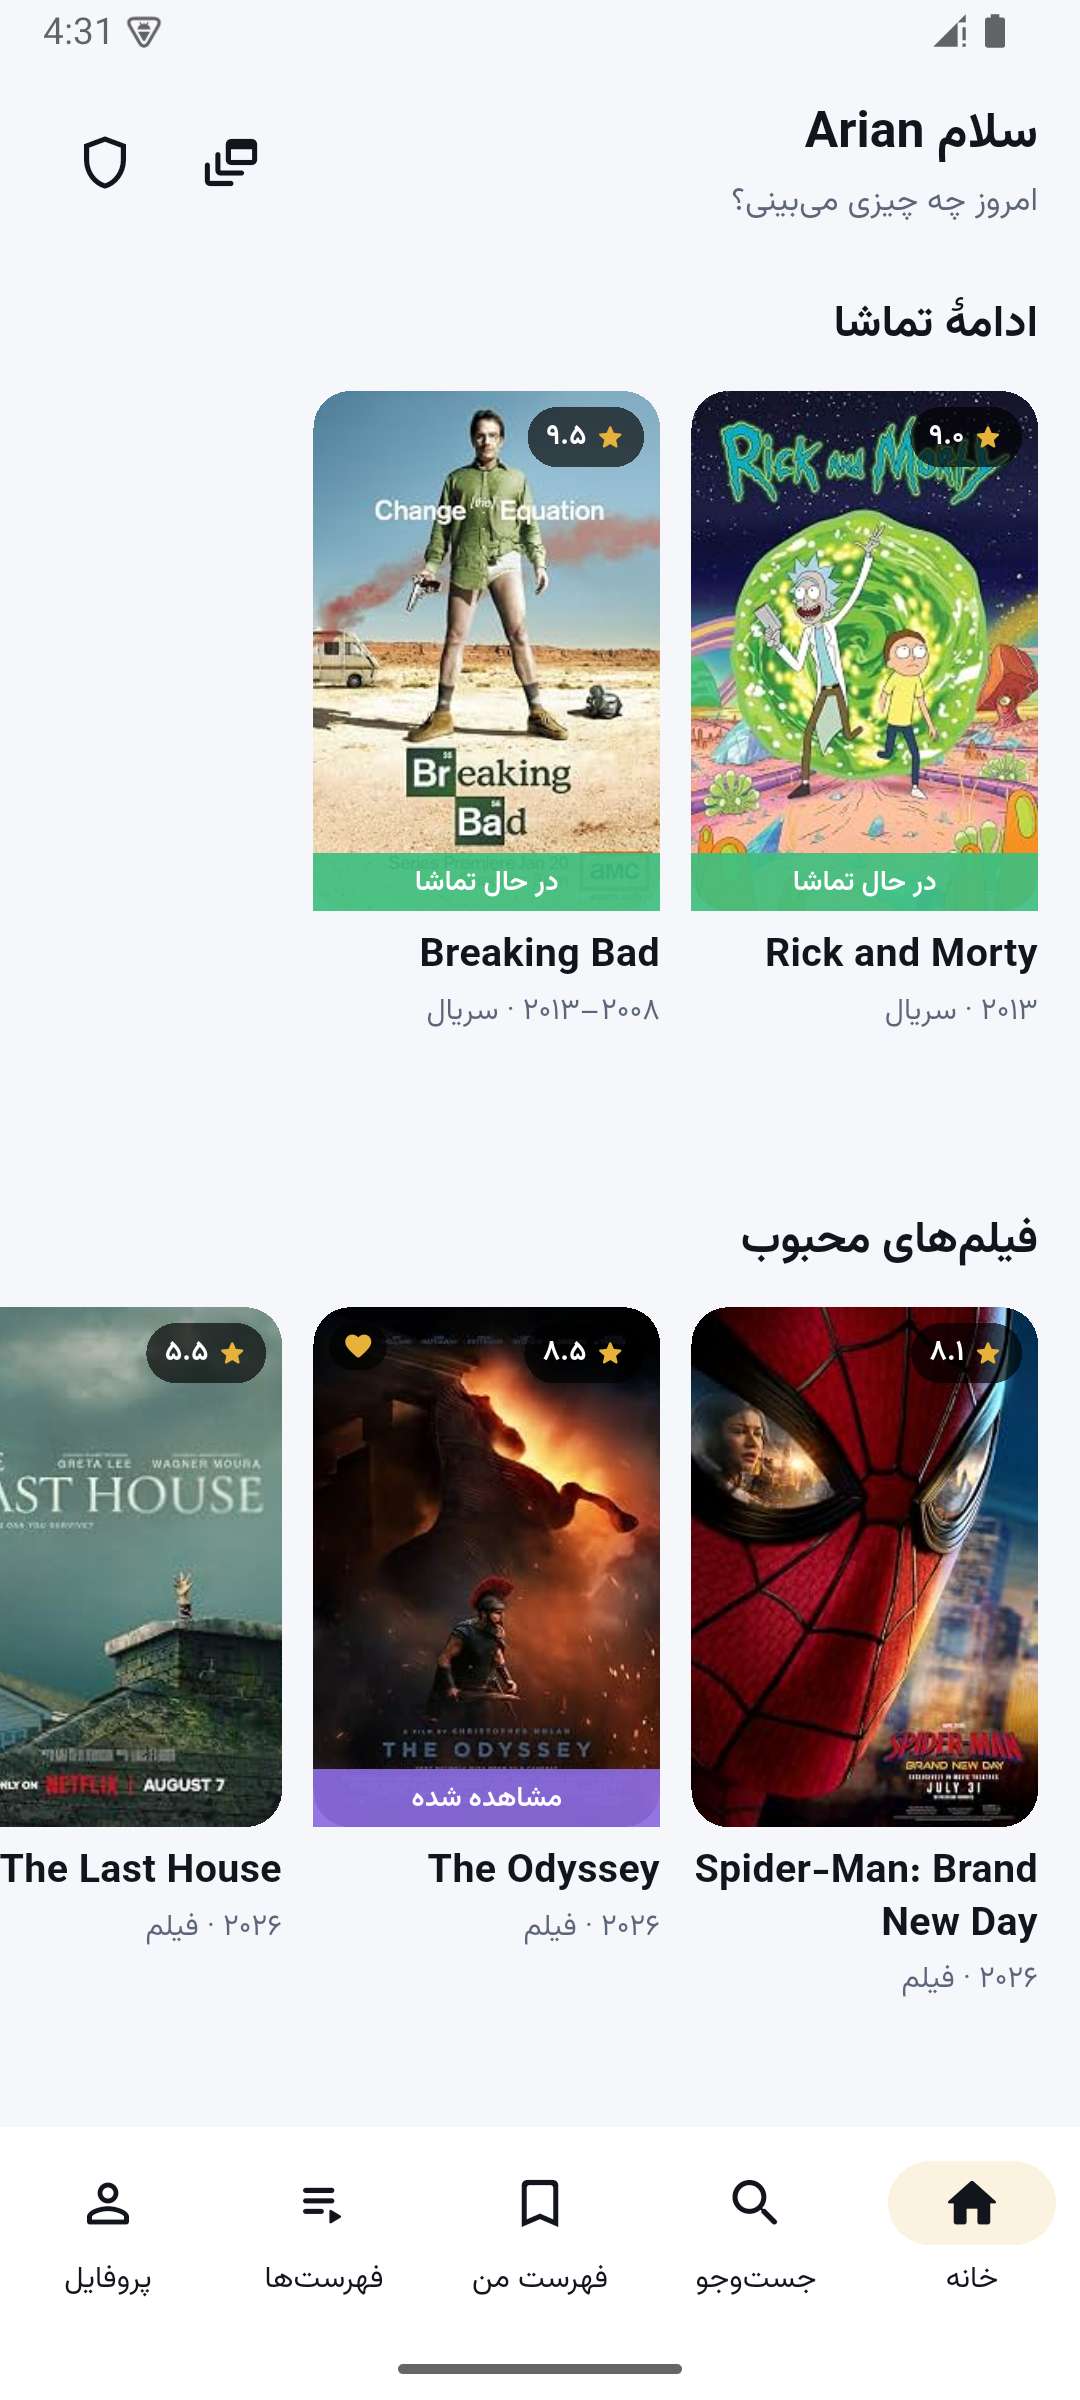
\includegraphics[width=0.3\textwidth]{docs/screenshots/13-offline.png}\hspace{0.4em}
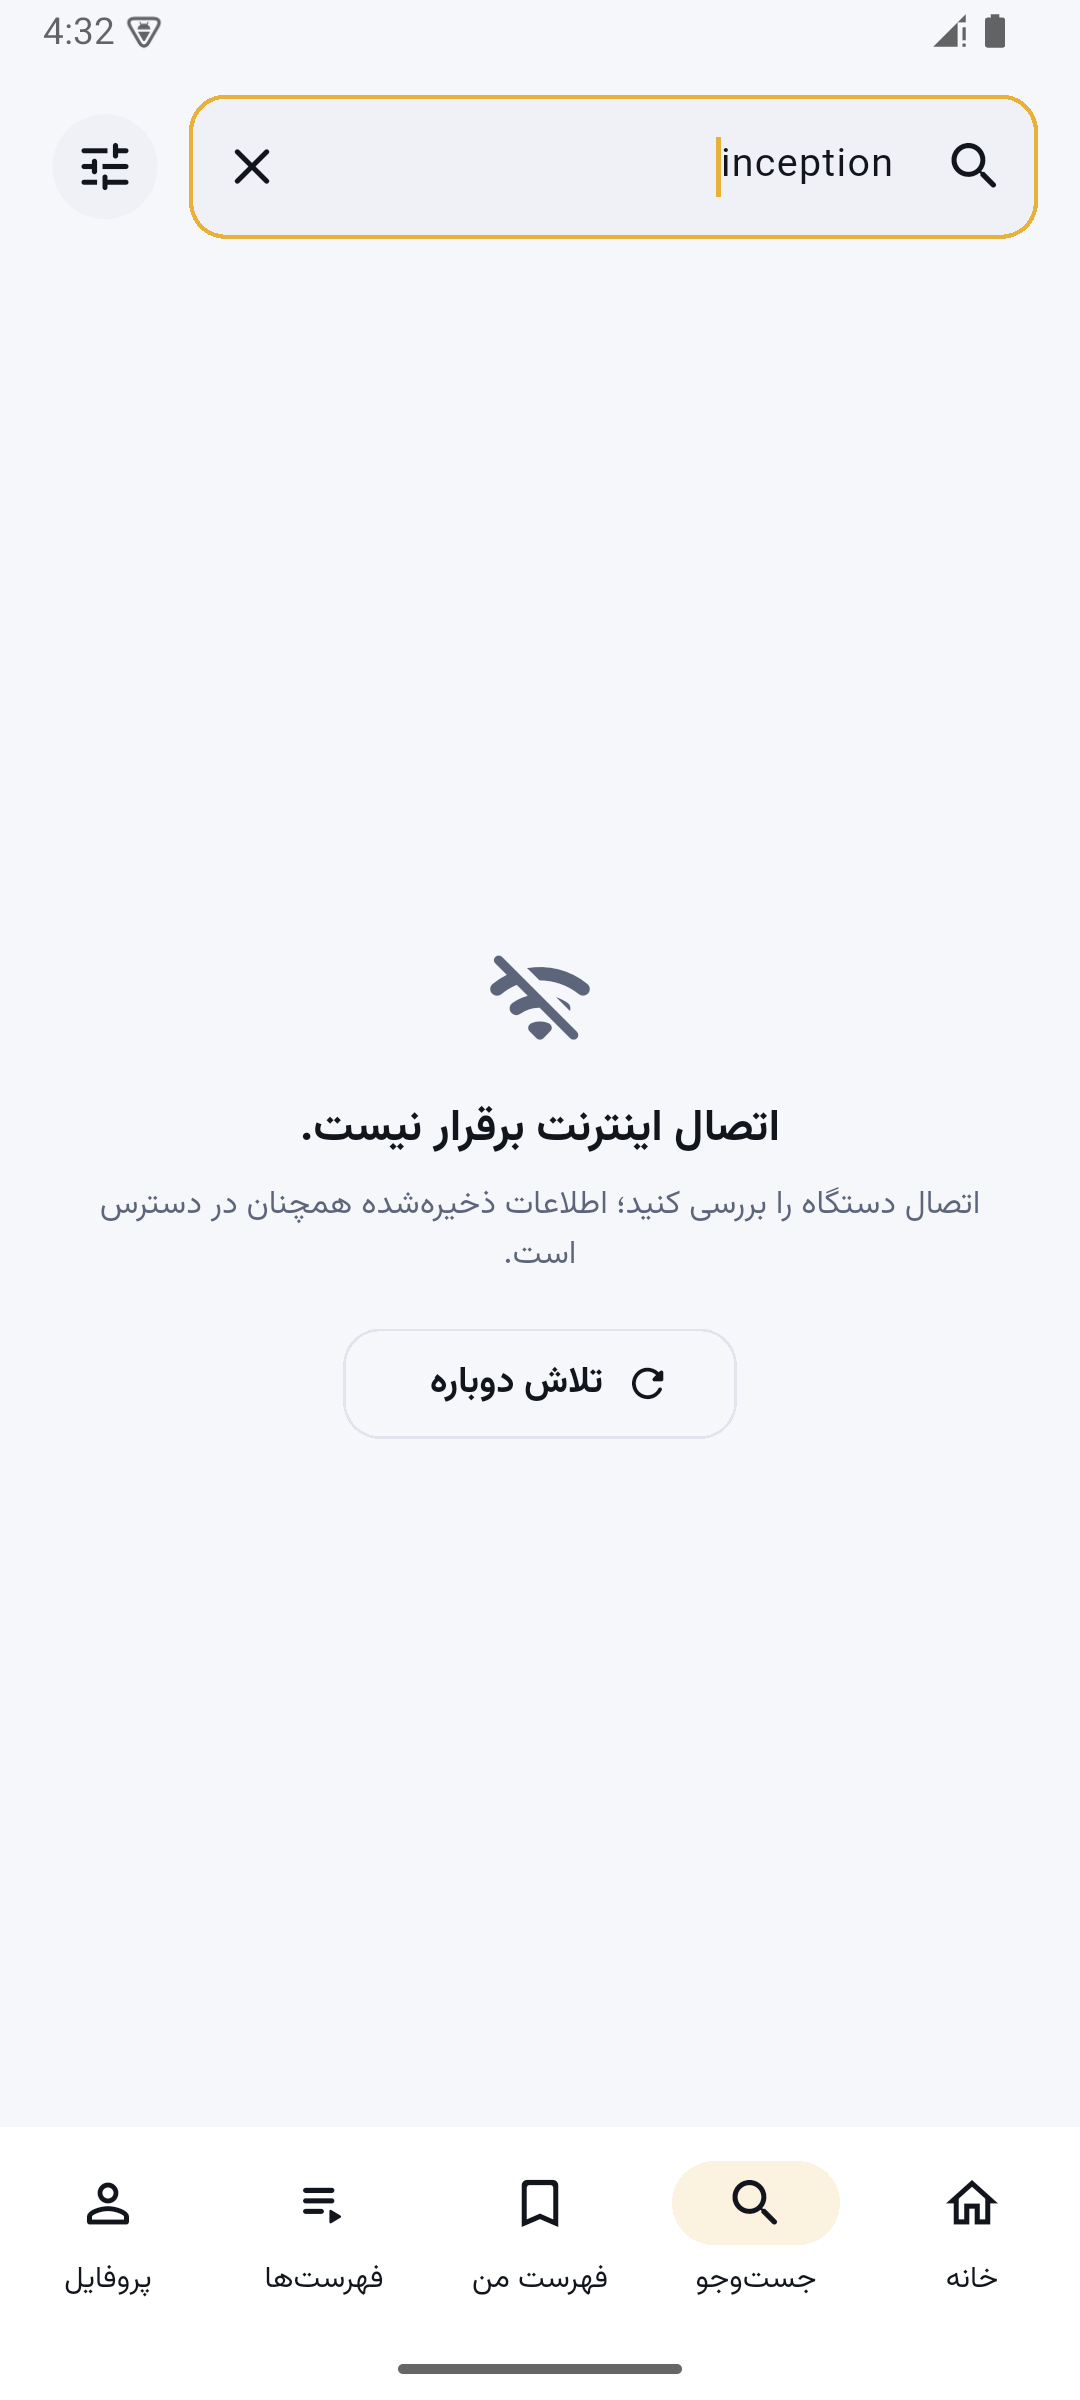
\includegraphics[width=0.3\textwidth]{docs/screenshots/14-offline-error.png}
\end{center}
\begin{center}
\small هر دو تصویر بدون اتصال گرفته شده‌اند: صفحهٔ اصلی از آینهٔ محلی بالا می‌آید، اما
جست‌وجو که ناچار است به شبکه برود پیام روشن می‌دهد (بخش \textenglish{۵.۲۰}).
\end{center}

\sub{تصویرها}

پوسترها در حافظهٔ نهان روی دیسک می‌مانند و در اندازه‌ای که واقعاً نمایش داده می‌شوند درخواست
می‌شوند، نه اندازهٔ اصلی. این هم مصرف اینترنت را پایین می‌آورد هم حافظه را (بخش \textenglish{۸.۸}).

\heading{صفحه‌ها و کار با برنامه}

\begin{center}
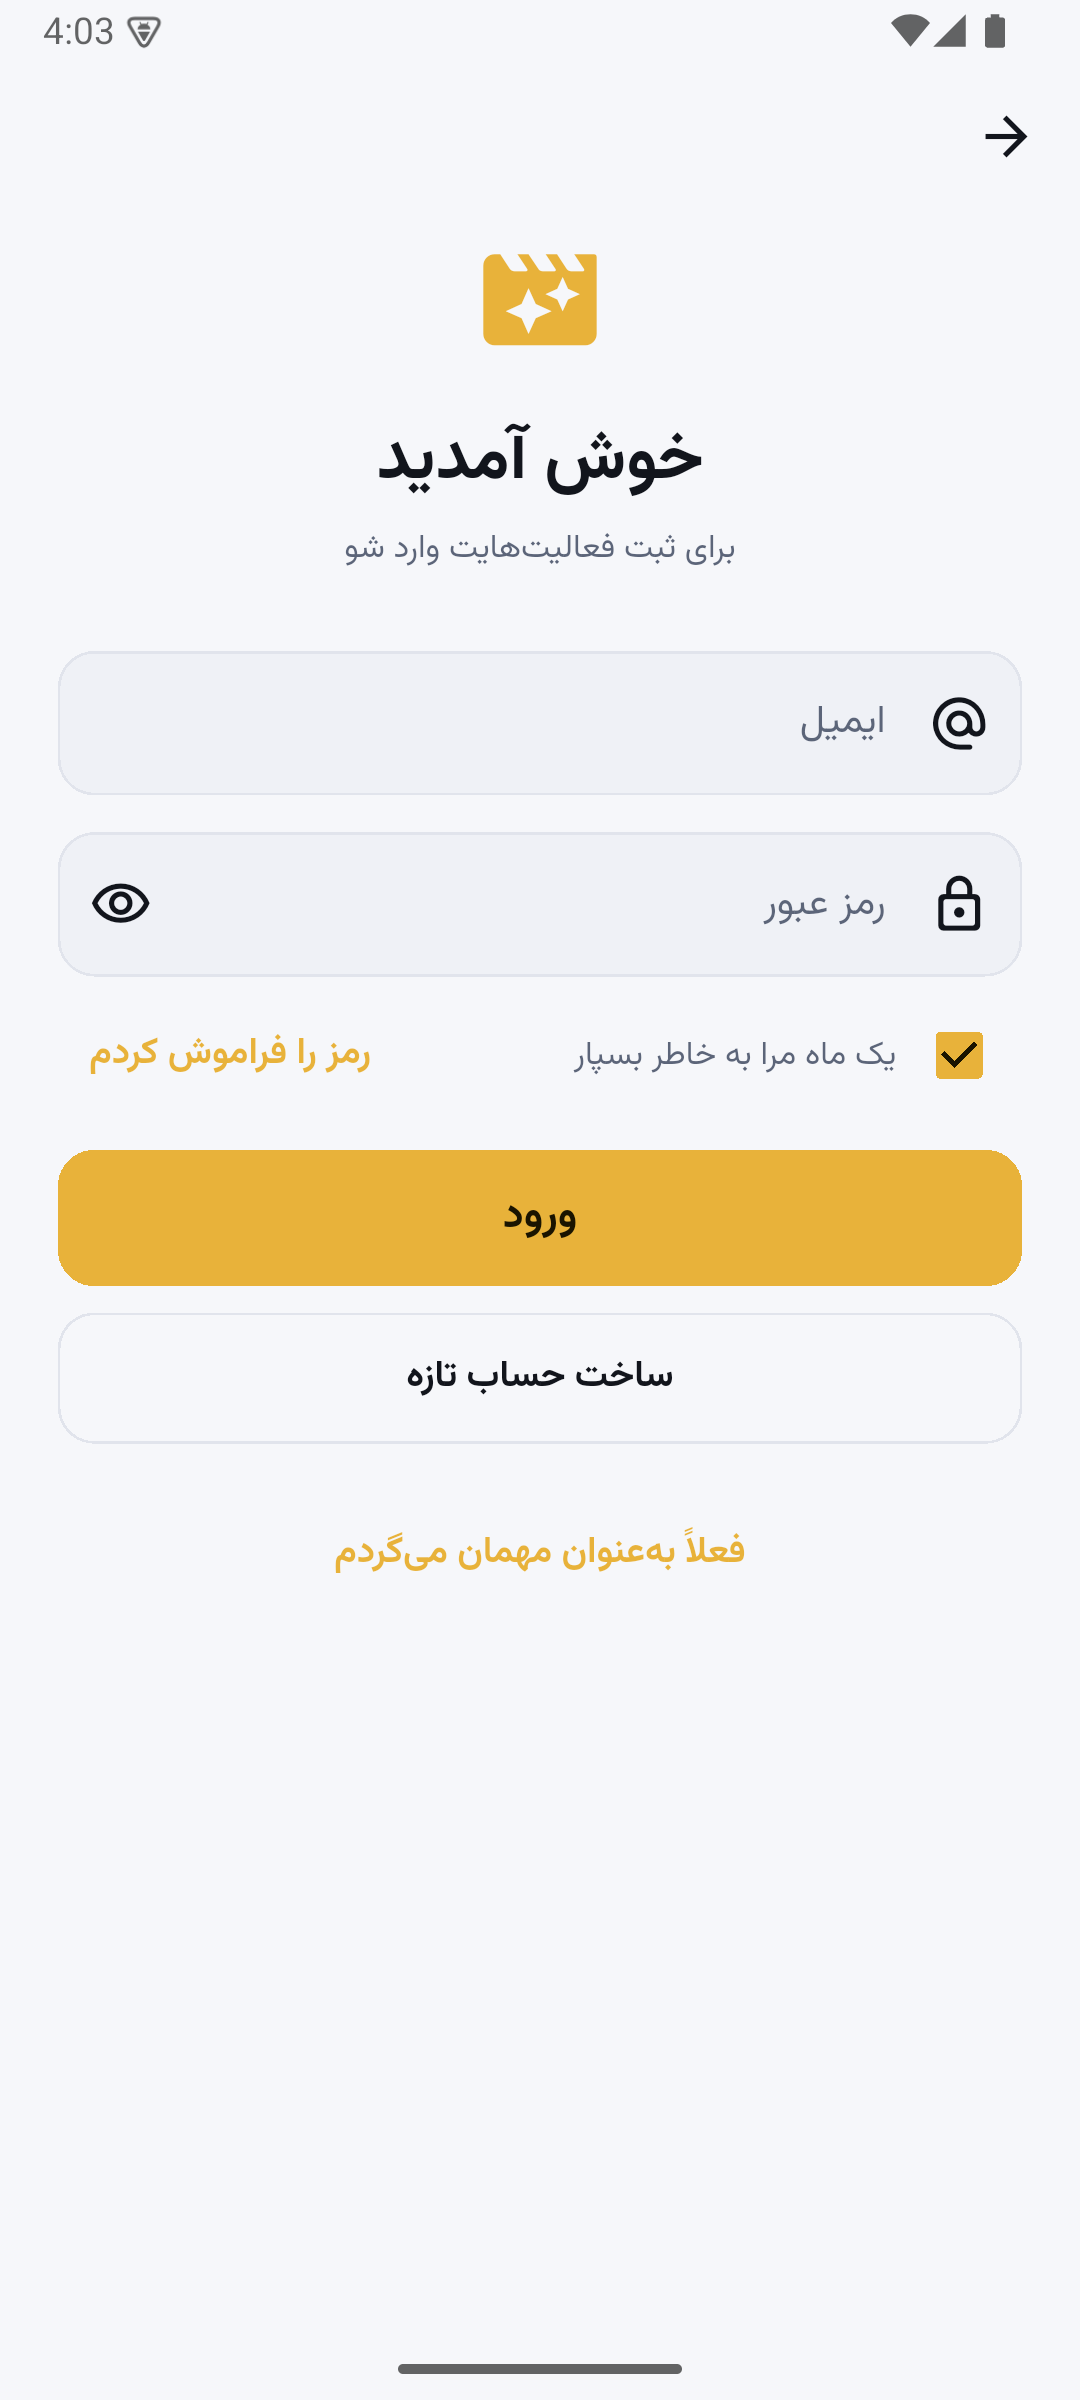
\includegraphics[width=0.3\textwidth]{docs/screenshots/02-login.png}\hspace{0.4em}
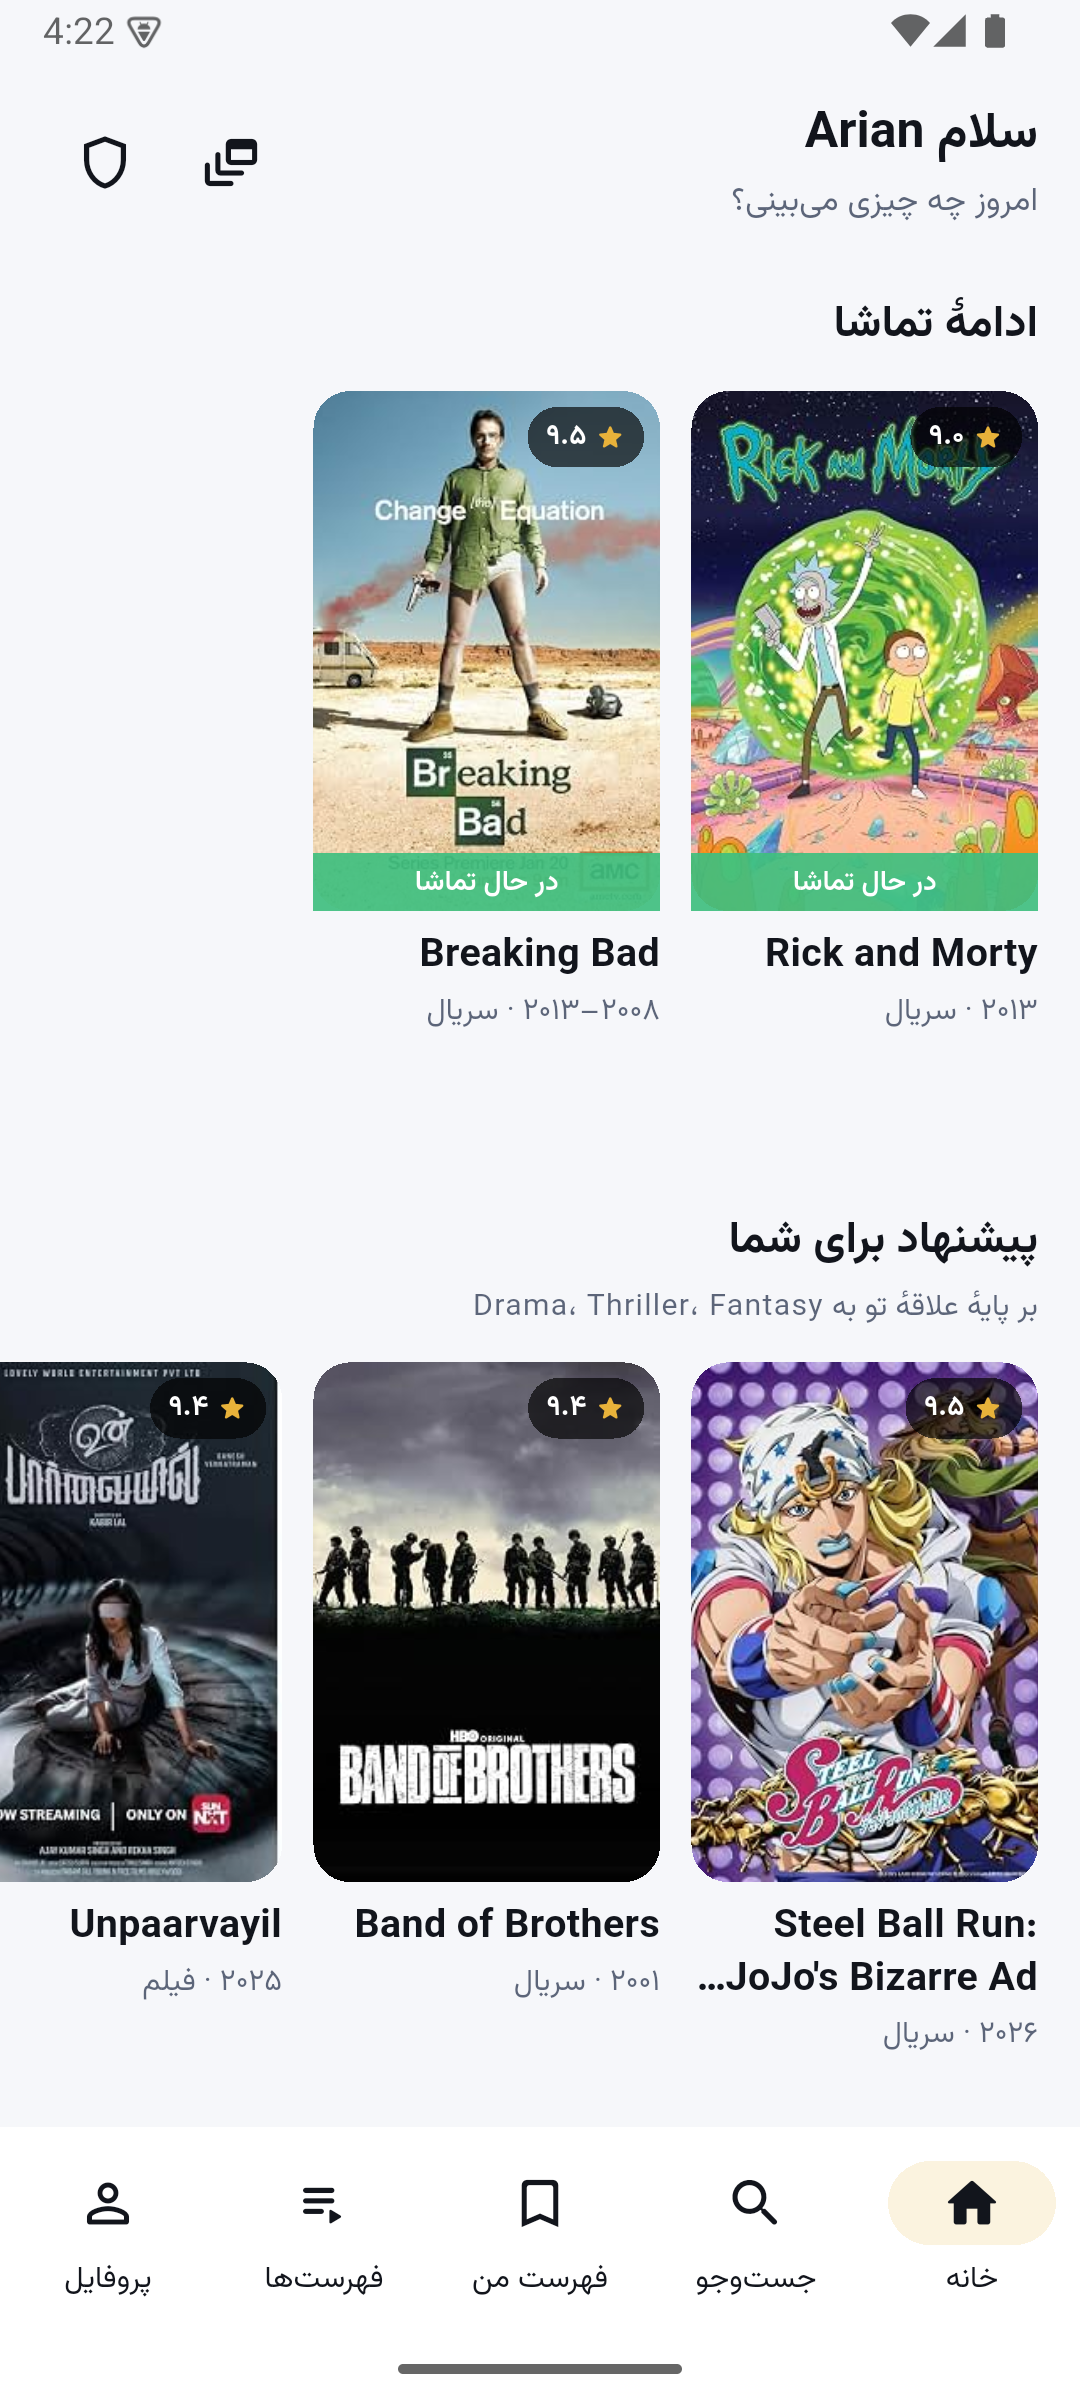
\includegraphics[width=0.3\textwidth]{docs/screenshots/01-home.png}\hspace{0.4em}
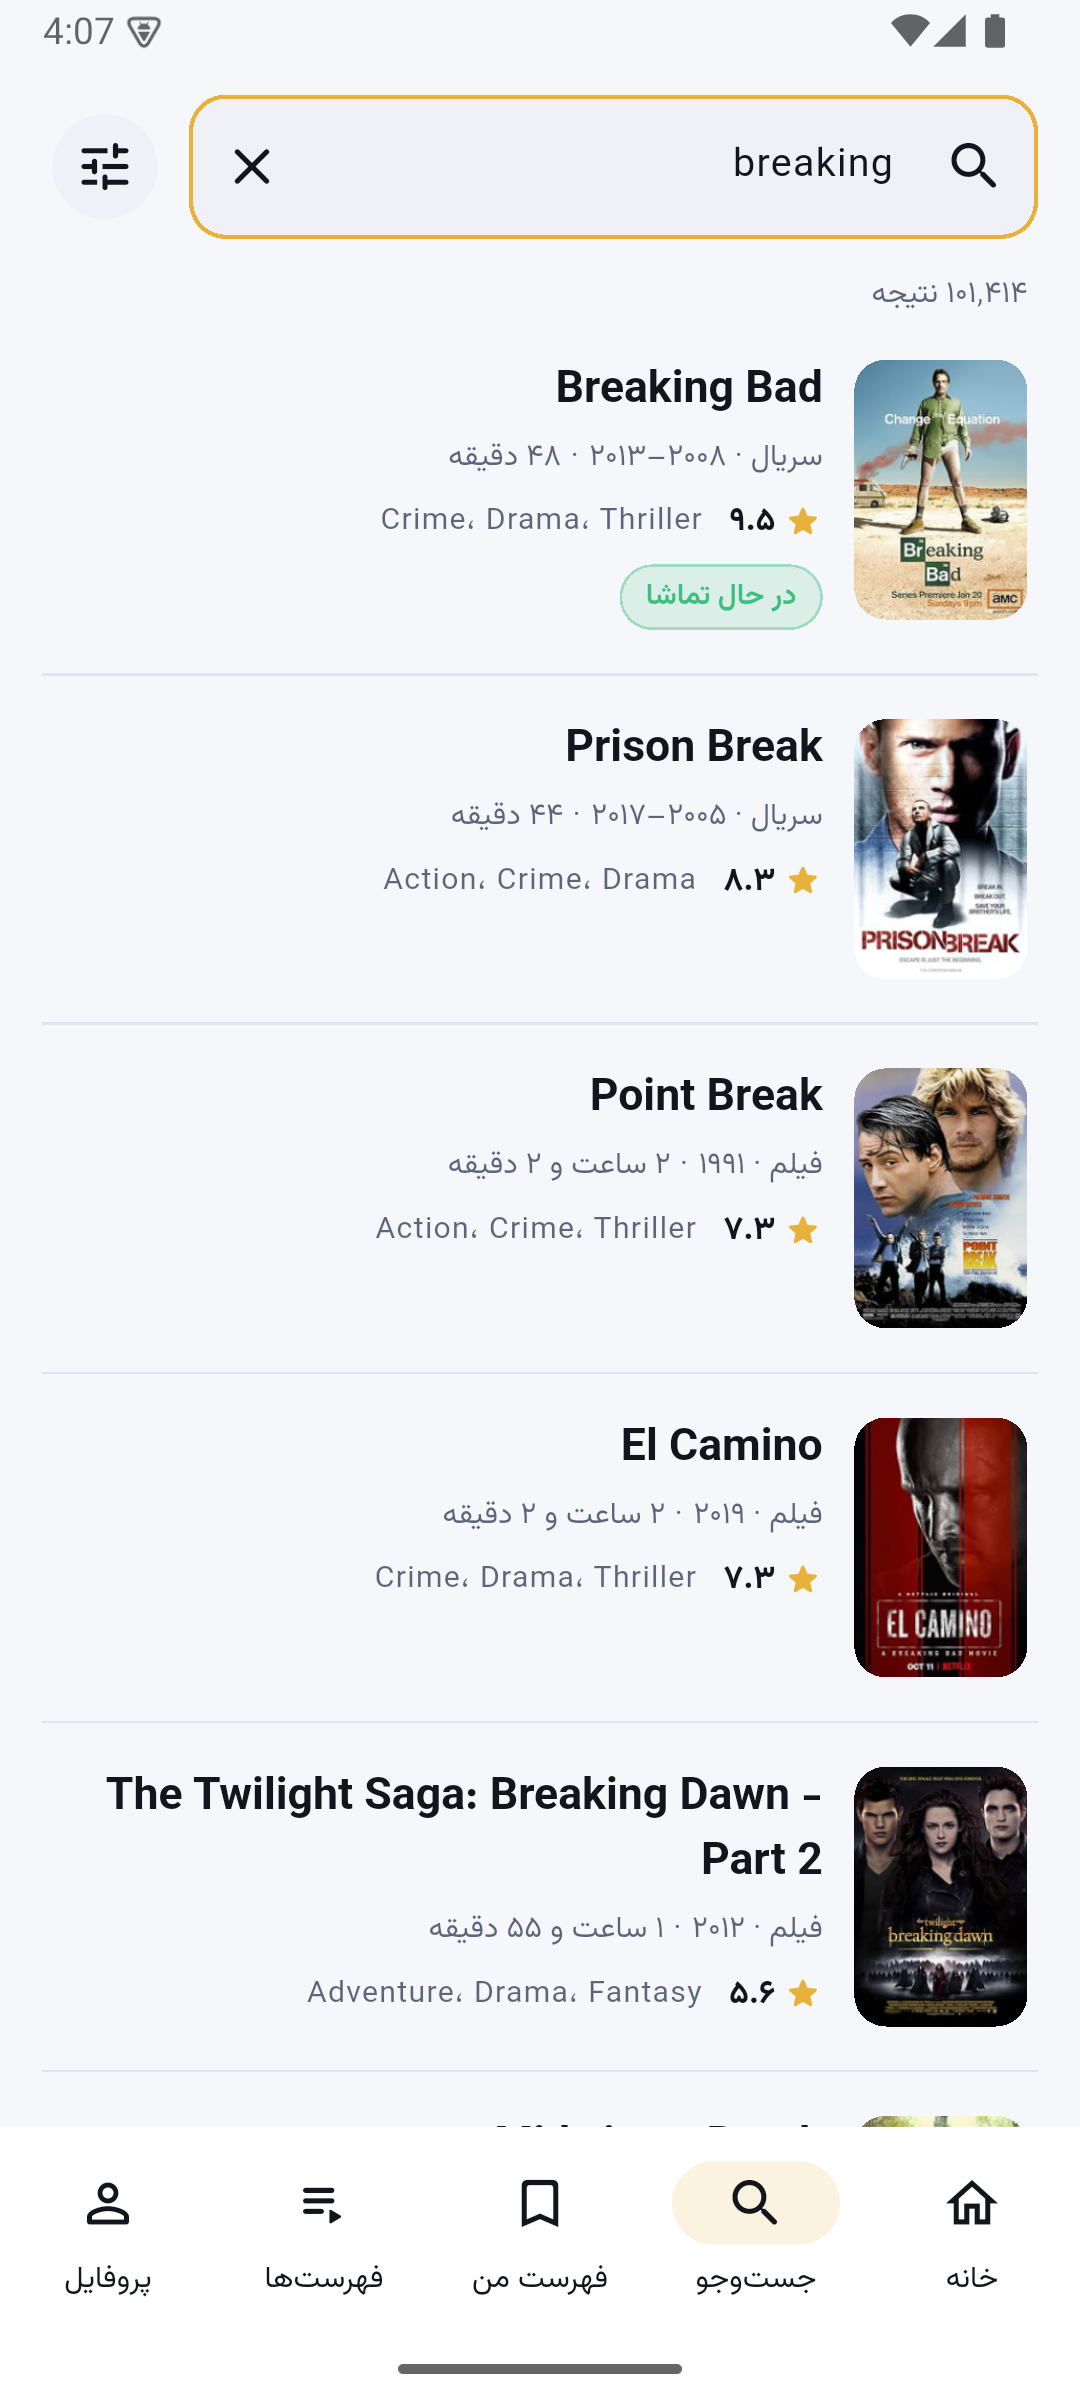
\includegraphics[width=0.3\textwidth]{docs/screenshots/04-search.png}
\end{center}
\begin{center}
\small ورود \enspace$\cdot$\enspace صفحهٔ اصلی \enspace$\cdot$\enspace جست‌وجو
\end{center}

\p{ورود و ثبت‌نام.} ثبت‌نام با نام، نام کاربری، ایمیل و رمز عبور انجام می‌شود؛ تصویر پروفایل و
توضیح کوتاه اختیاری‌اند. ایمیل و نام کاربری تکراری همان‌جا رد می‌شوند. اگر رمز یادتان برود،
از «فراموشی رمز» می‌شود آن را بازیابی کرد.

کاربر مهمان بدون ثبت‌نام هم می‌تواند جست‌وجو کند، صفحهٔ آثار را ببیند و آثار محبوب و فصل‌ها و
قسمت‌ها را مرور کند. برای ثبت هر فعالیتی (وضعیت، امتیاز، نظر، فهرست) ورود لازم است.

\p{صفحهٔ اصلی.} ردیف‌های فیلم‌های محبوب، سریال‌های محبوب، آثار جدید، آثار با امتیاز بالا و
سریال‌های برتر. برای کاربری که فعالیتی داشته، یک ردیف «پیشنهاد برای شما» هم می‌آید که بر پایهٔ
ژانرهای واقعی خودش ساخته می‌شود. تا وقتی سیگنالی نباشد این ردیف اصلاً نشان داده نمی‌شود تا
همان ردیف محبوب‌ها دوباره تکرار نشود.

\p{جست‌وجو.} دست‌کم بر اساس نام اثر کار می‌کند و پالایه‌های ژانر، سال، نوع اثر و نام
بازیگر یا کارگردان هم دارد. تایپ که می‌کنید درخواست بلافاصله نمی‌رود؛ کمی صبر می‌کند تا دست
کاربر بایستد و بعد یک درخواست بفرستد.

\begin{center}
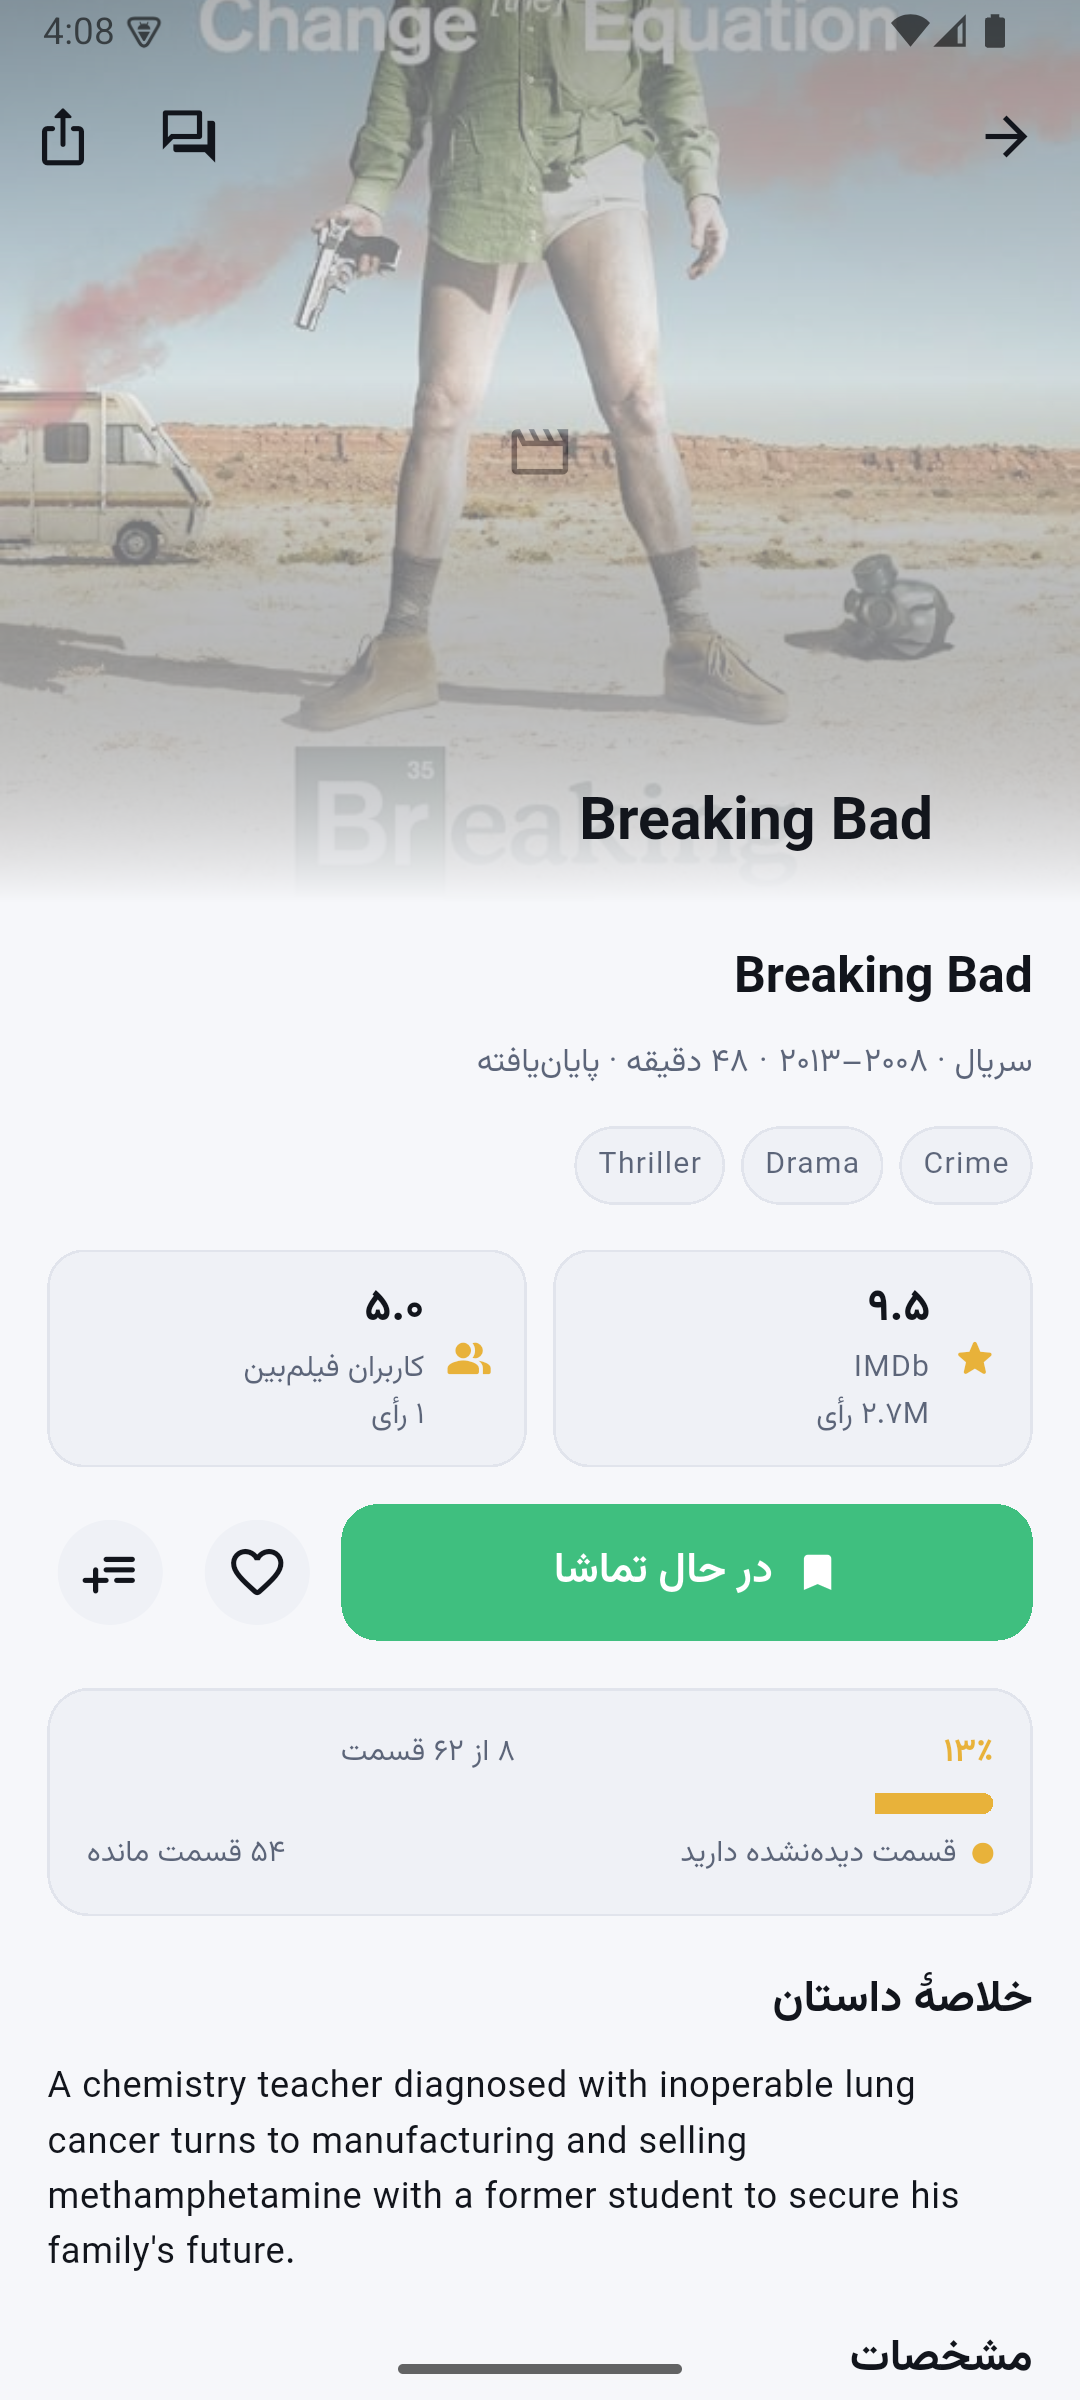
\includegraphics[width=0.3\textwidth]{docs/screenshots/05-title-detail.png}\hspace{0.4em}
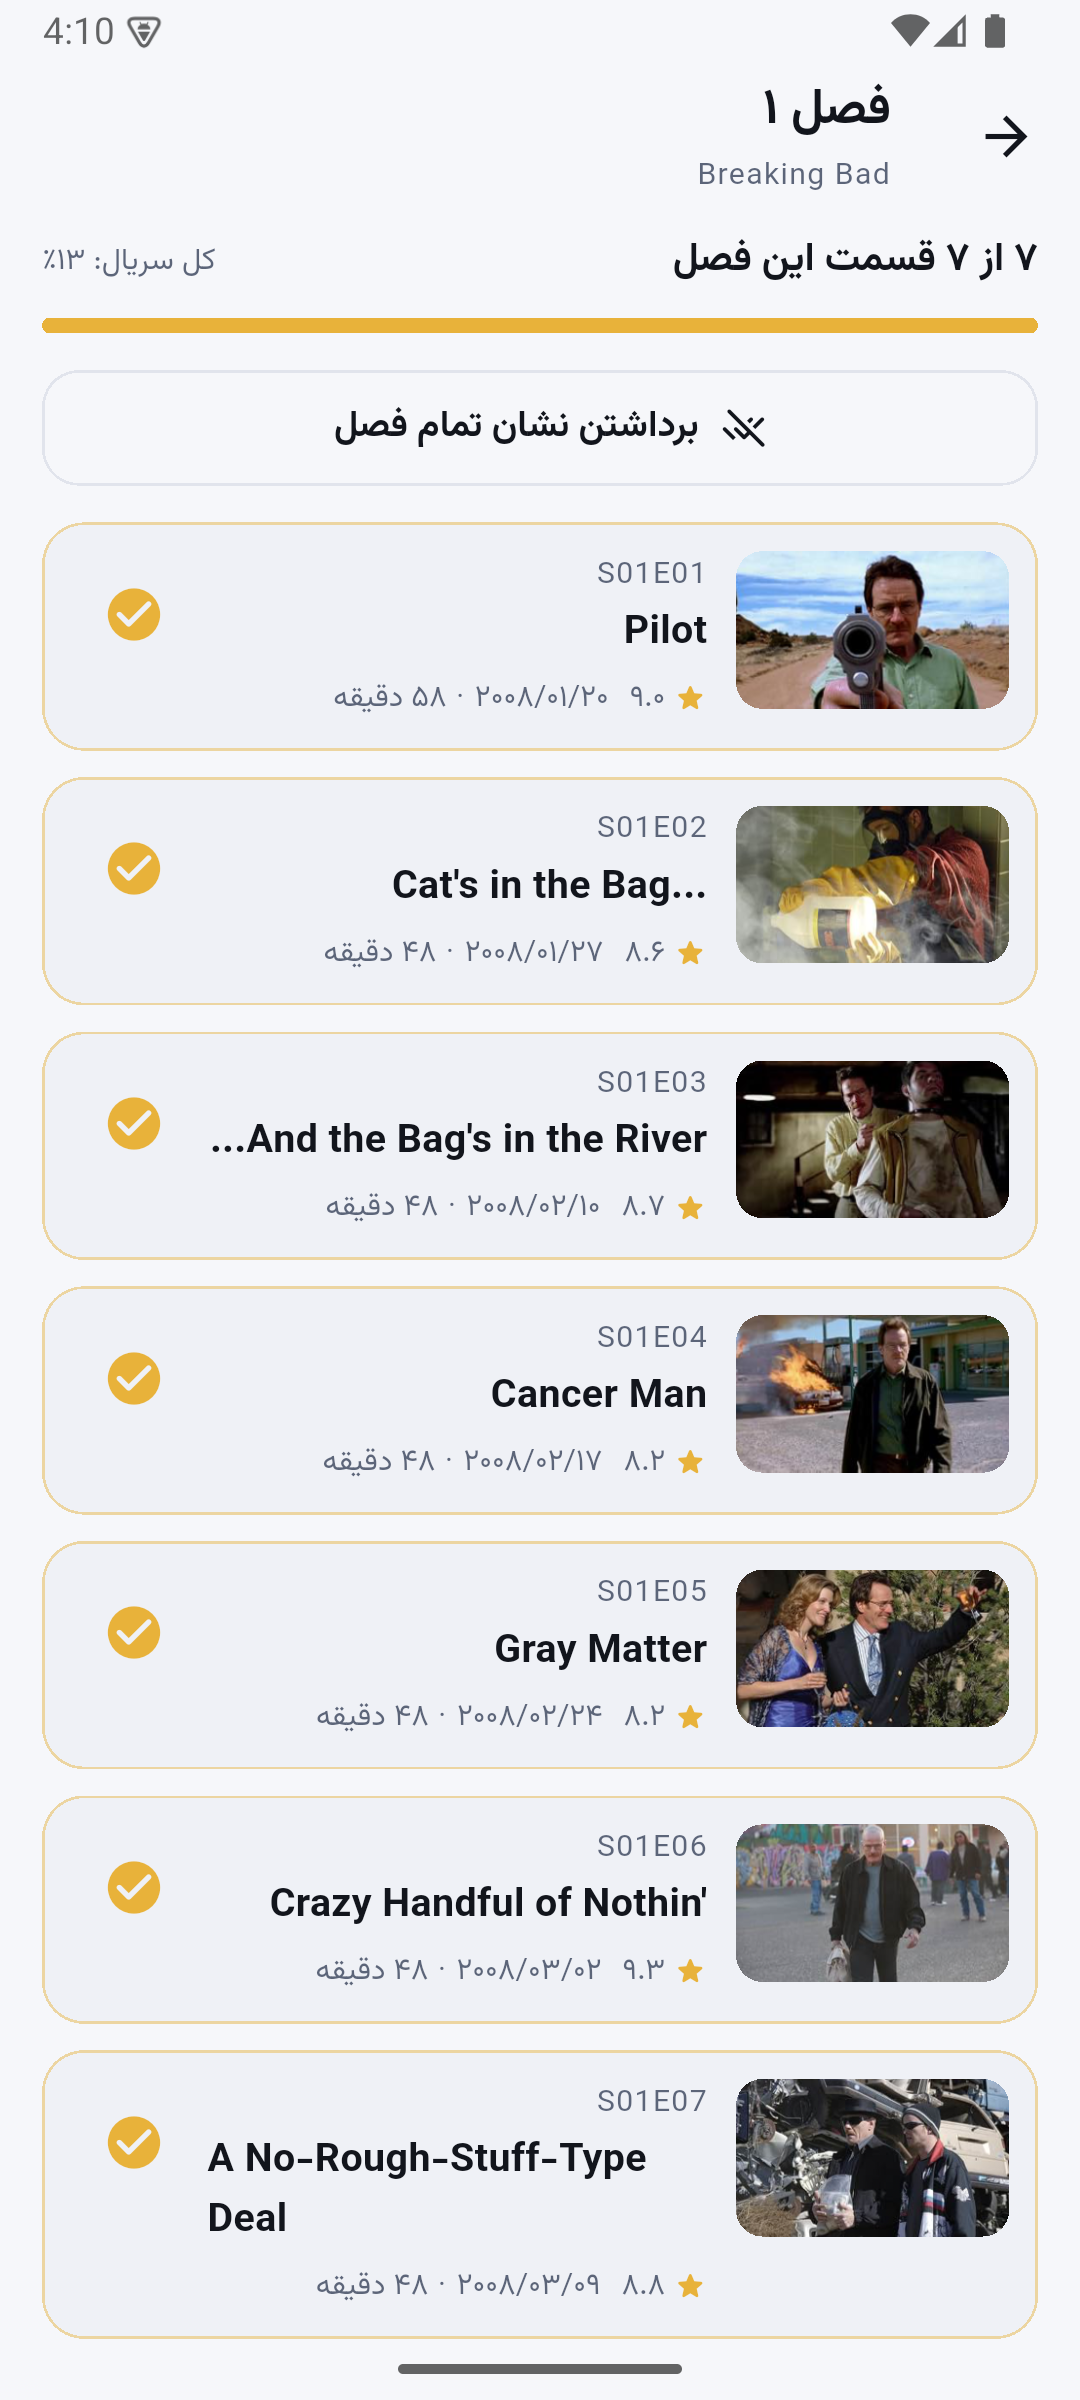
\includegraphics[width=0.3\textwidth]{docs/screenshots/07-episodes.png}\hspace{0.4em}
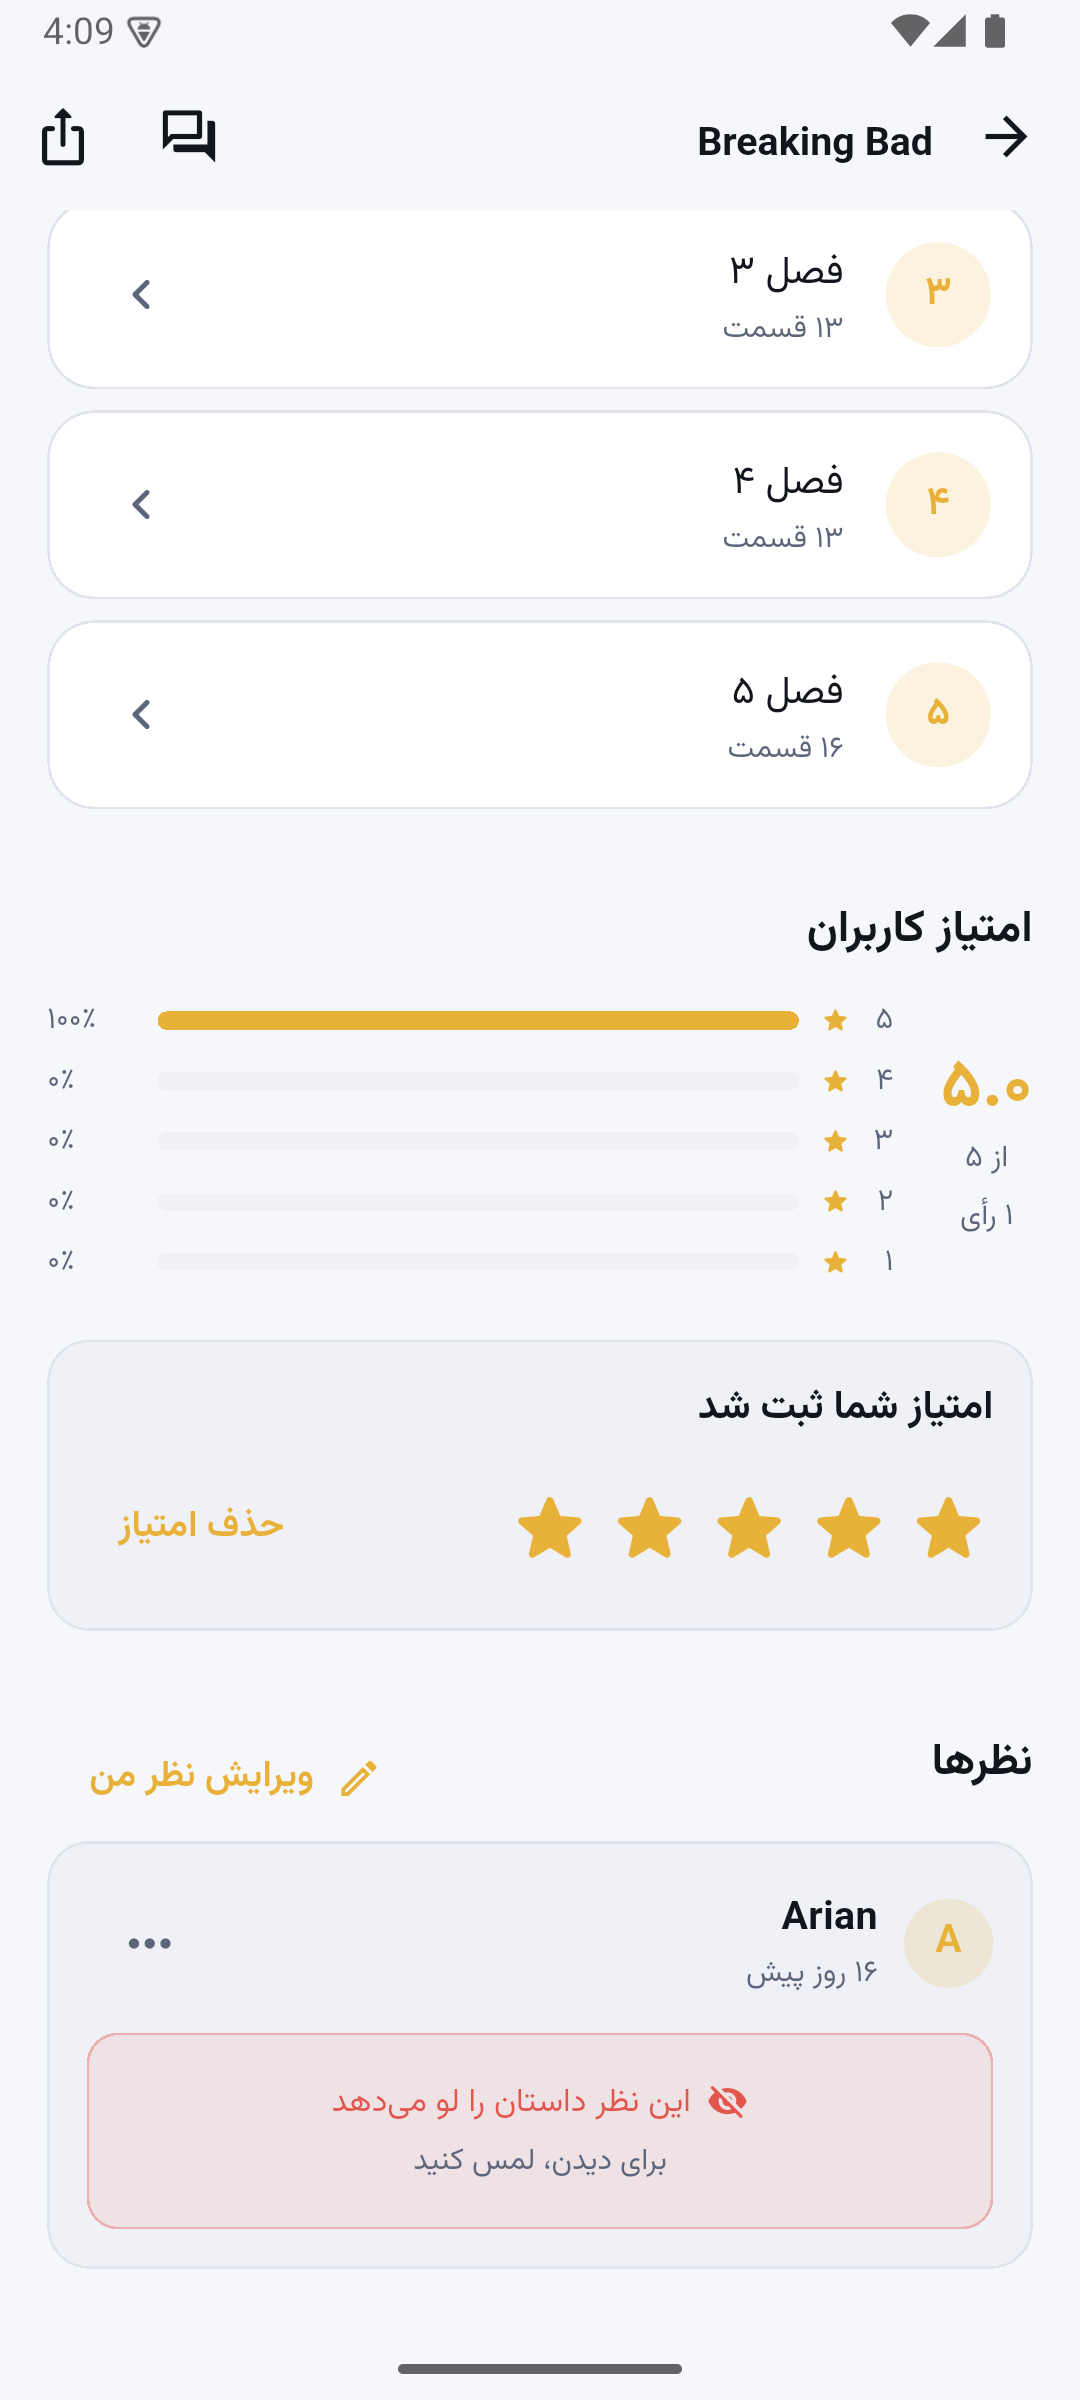
\includegraphics[width=0.3\textwidth]{docs/screenshots/08-rating-review.png}
\end{center}
\begin{center}
\small صفحهٔ اثر \enspace$\cdot$\enspace قسمت‌ها \enspace$\cdot$\enspace امتیاز و نظر
\end{center}

\p{صفحهٔ اثر.} برای فیلم: نام، نام اصلی، پوستر، خلاصهٔ داستان، سال، مدت زمان، ژانر، کشور
سازنده، کارگردان، بازیگران، امتیاز \en{IMDb} و امتیاز کاربران خود برنامه. برای سریال به‌جای
مدت زمان، سال شروع و پایان پخش، وضعیت پخش، تعداد فصل‌ها و تعداد قسمت‌ها می‌آید.

\p{فصل‌ها و قسمت‌ها.} هر قسمت شمارهٔ فصل، شمارهٔ قسمت، عنوان، تاریخ پخش، مدت زمان، خلاصه و
وضعیت دیده‌شدن دارد. می‌شود یک قسمت را تیک زد یا کل یک فصل را یک‌جا علامت زد. تعداد
دیده‌شده و باقی‌مانده همان‌جا حساب می‌شود.

\p{امتیاز و نظر.} امتیاز از یک تا پنج ستاره است و توزیع درصدی ستاره‌ها زیرش نشان داده می‌شود.
امتیاز قبلی قابل ویرایش است. نظر شامل متن، نام و تصویر کاربر، تاریخ ثبت و وضعیت اسپویل است؛
نظر اسپویل‌دار اول پوشانده می‌شود و فقط با زدن روی آن باز می‌شود.

\begin{center}
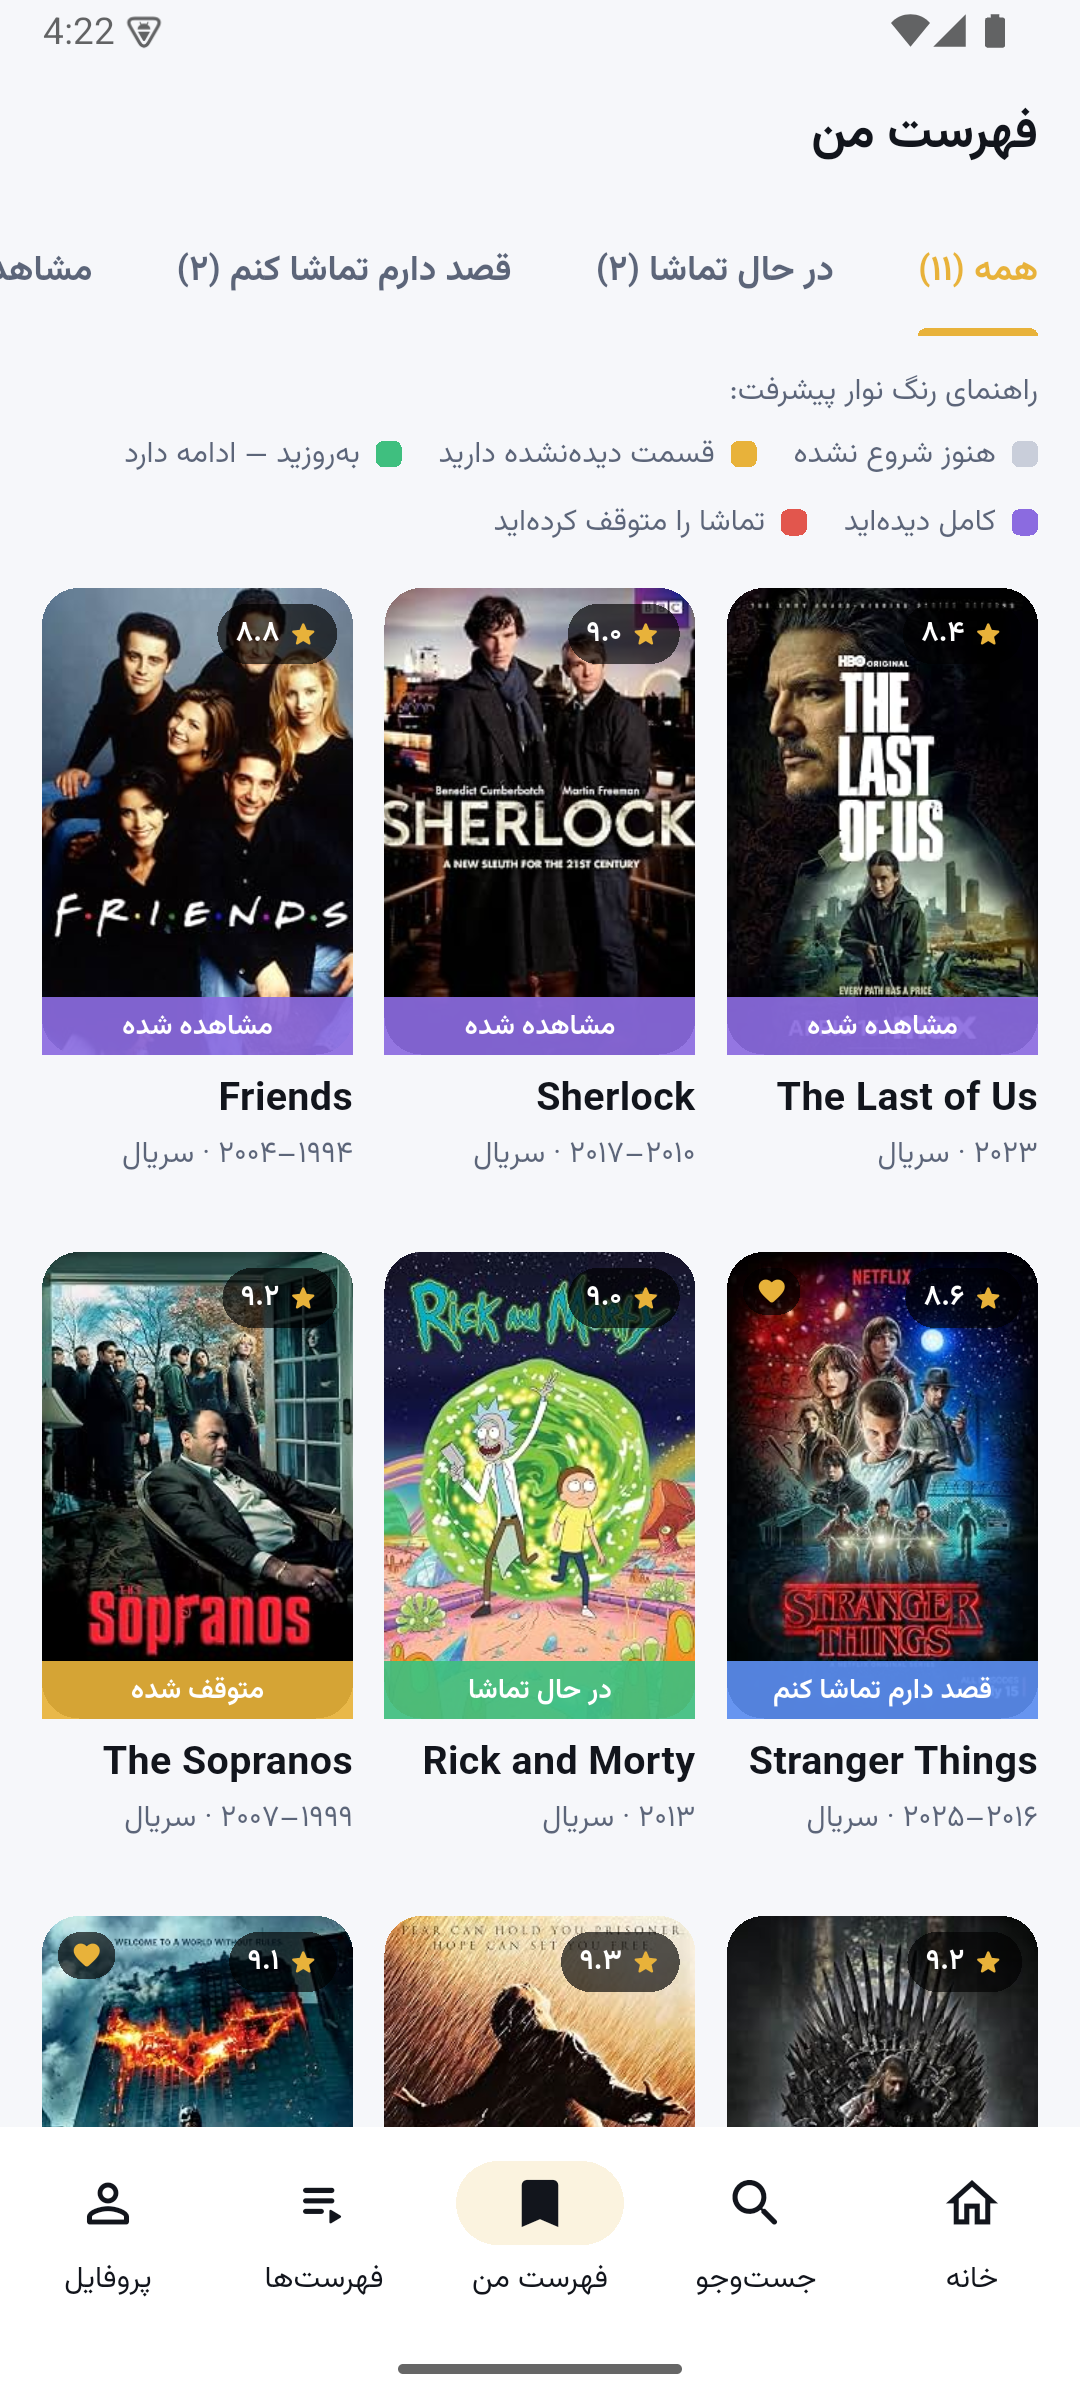
\includegraphics[width=0.3\textwidth]{docs/screenshots/09-watchlist.png}\hspace{0.4em}
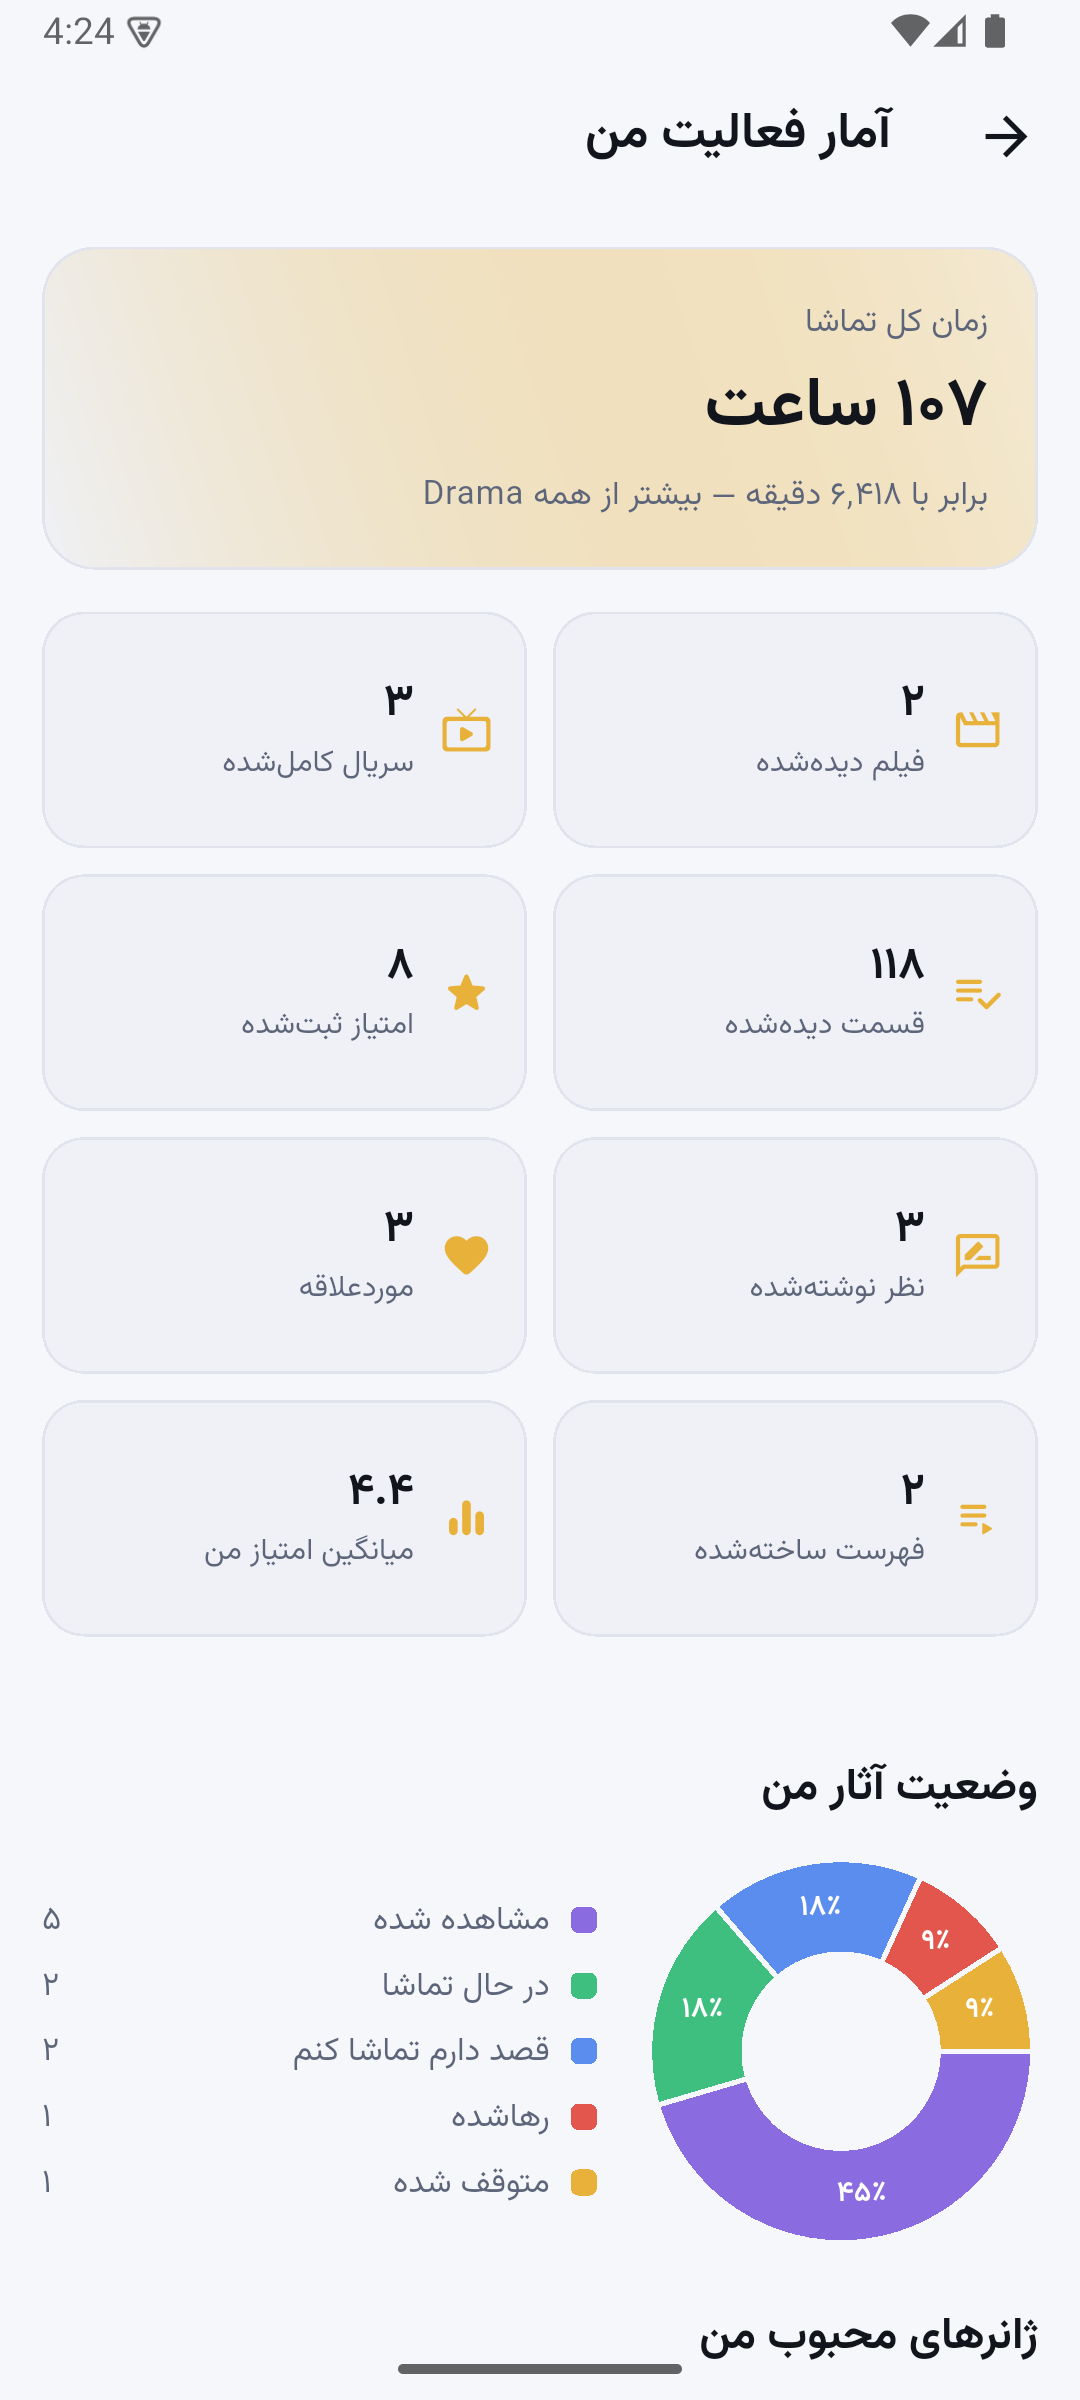
\includegraphics[width=0.3\textwidth]{docs/screenshots/11-stats.png}\hspace{0.4em}
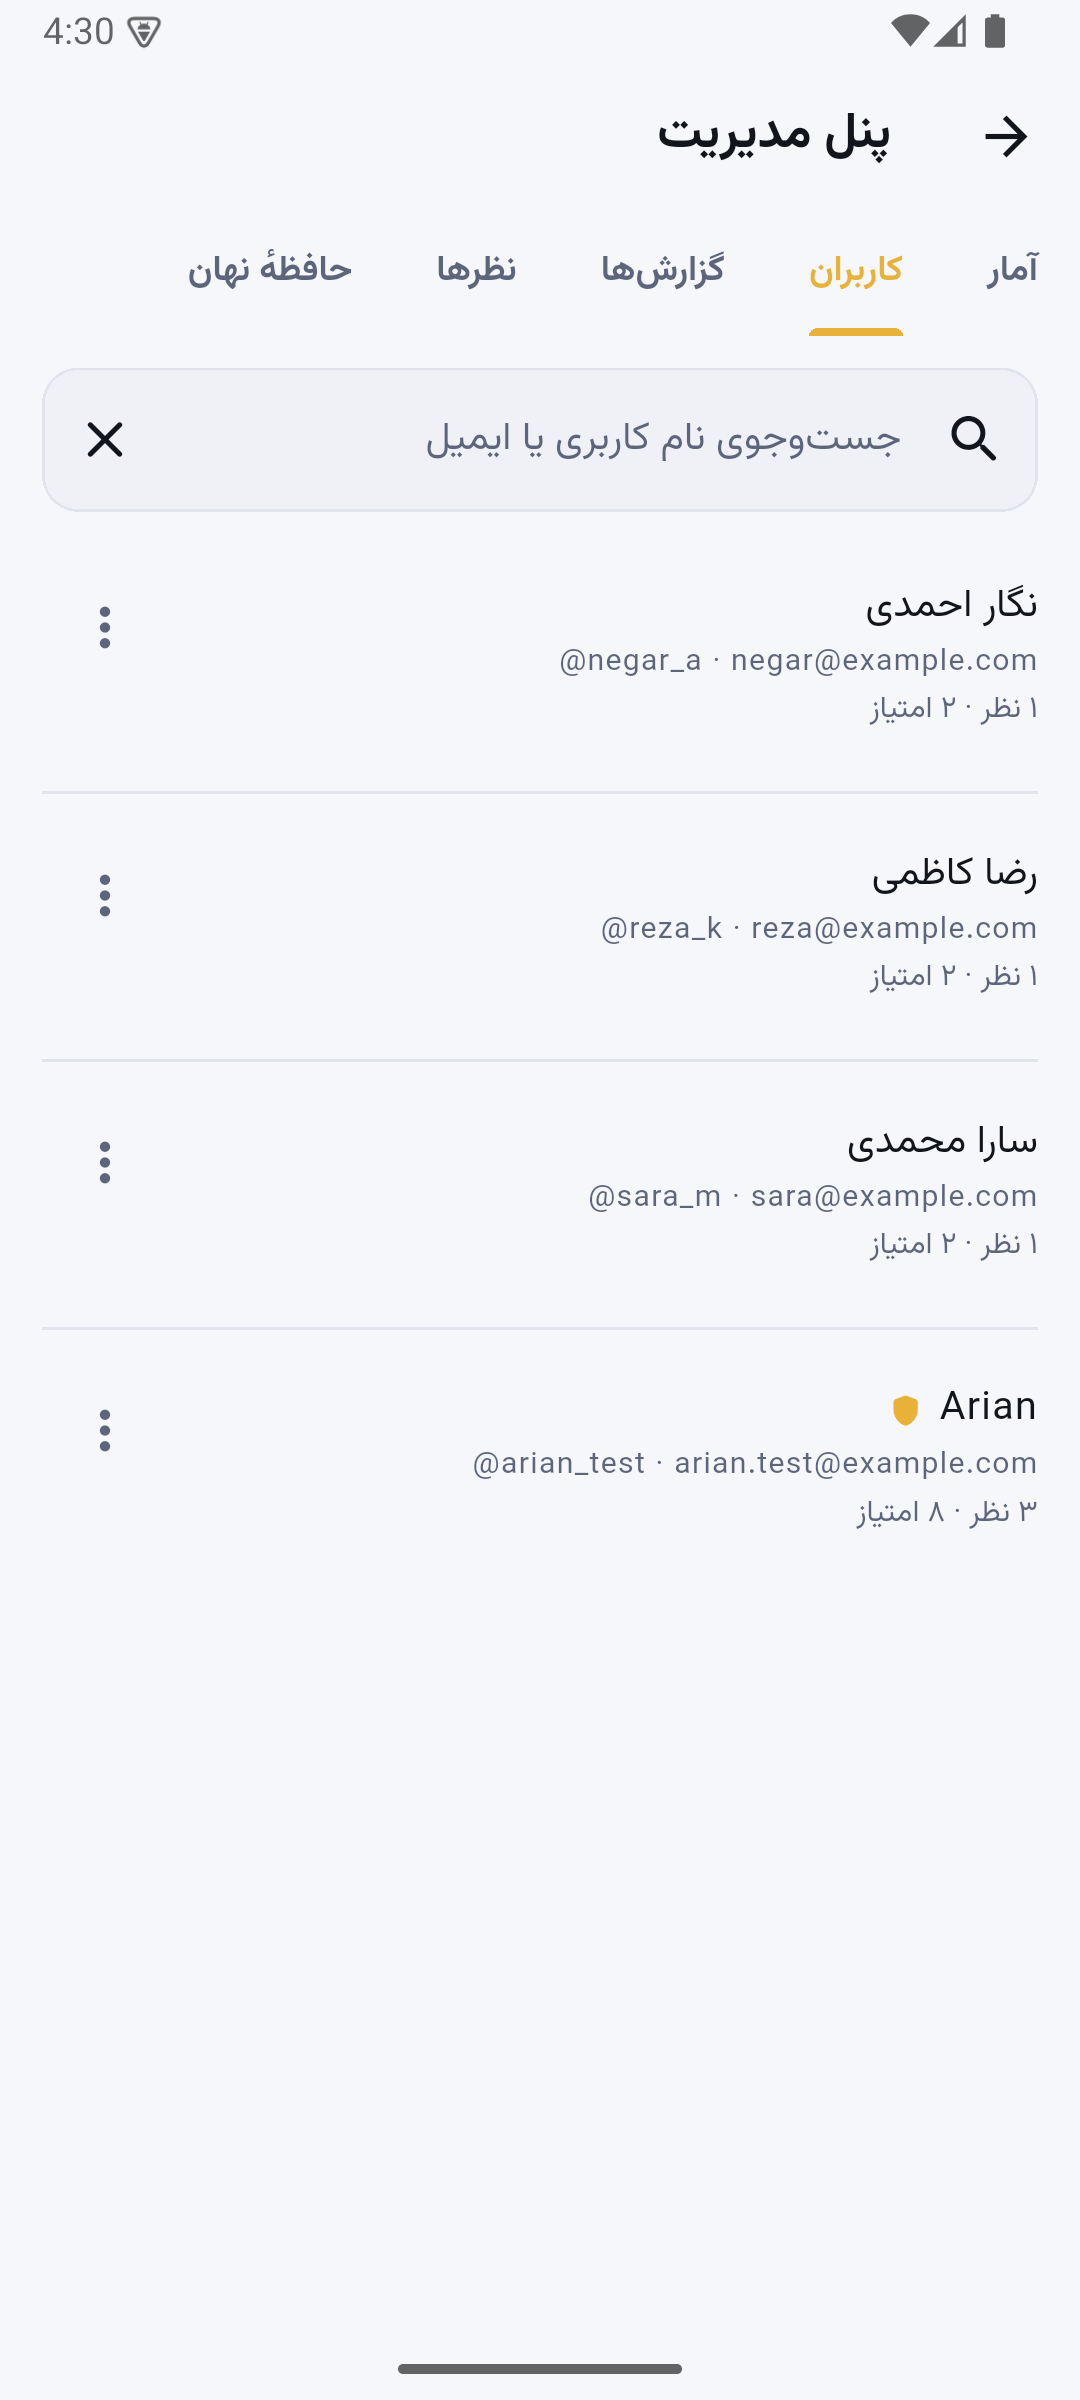
\includegraphics[width=0.3\textwidth]{docs/screenshots/12-admin.png}
\end{center}
\begin{center}
\small فهرست تماشا \enspace$\cdot$\enspace آمار فعالیت \enspace$\cdot$\enspace پنل مدیر
\end{center}

\p{فهرست تماشا و فهرست‌های شخصی.} پنج وضعیت داریم: قصد دارم تماشا کنم، در حال تماشا، مشاهده‌شده،
متوقف‌شده و رهاشده. «موردعلاقه» کنار این‌ها یک پرچم جداست. علاوه بر این‌ها کاربر می‌تواند
فهرست دلخواه بسازد («بهترین فیلم‌های اکشن»، «فیلم‌هایی که باید ببینم») و آثار را به آن اضافه یا
از آن حذف کند.

\p{آمار فعالیت.} تعداد فیلم‌های دیده‌شده، سریال‌های دیده‌شده، قسمت‌های دیده‌شده، مجموع زمان
تقریبی تماشا، ژانر موردعلاقه و میانگین امتیازهای ثبت‌شده.

\p{پنل مدیر.} مدیر سیستم می‌تواند کاربرها را ببیند و مدیریت کند، نظرهای نامناسب را حذف کند،
گزارش‌های کاربرها را بررسی کند و آمار کلی سامانه را ببیند.

\heading{نوار پیشرفت و رنگ‌بندی‌اش}

درصد پیشرفت تماشای سریال هم به‌صورت عدد و هم به‌صورت نواری زیر پوستر نشان داده می‌شود که عرضش
به همان نسبت پر می‌شود. رنگ نوار روی سرور حساب می‌شود تا همهٔ کلاینت‌ها یک چیز نشان بدهند:

\begin{center}
\begin{tabular}{|l|p{9cm}|}
\hline
\textbf{رنگ} & \textbf{یعنی} \\
\hline
بی‌رنگ & هنوز هیچ قسمتی دیده نشده \\
\hline
زرد & قسمت دیده‌نشده باقی مانده \\
\hline
سبز & همه را دیده‌ای، ولی سریال ادامه دارد و قسمت جدید می‌آید \\
\hline
بنفش & همه را دیده‌ای و سریال تمام شده \\
\hline
قرمز & وسط کار متوقف کرده‌ای و کامل ندیده‌ای \\
\hline
\end{tabular}
\end{center}

\heading{پوشش خواسته‌های صورت پروژه}

\sub{بخش ۵ — نیازمندی‌های کاربردی}

\begin{center}
\begin{longtable}{|l|p{9.3cm}|}
\hline
\textbf{بند} & \textbf{کجا پیاده شده} \\
\hline
\endfirsthead
\hline
\textbf{بند} & \textbf{کجا پیاده شده} \\
\hline
\endhead
\textenglish{۵.۱} ثبت‌نام & \en{register\_screen.dart} + \en{routes/auth.py} \\
\hline
\textenglish{۵.۲} ورود و خروج & \en{login\_screen.dart}، نشست ۳۰ روزه \\
\hline
\textenglish{۵.۳} بازیابی رمز & \en{forgot\_password\_screen.dart} \\
\hline
\textenglish{۵.۴} مدیریت پروفایل & \en{screens/profile/} \\
\hline
\textenglish{۵.۵} جست‌وجو & \en{search\_screen.dart} \\
\hline
\textenglish{۵.۶} جزئیات فیلم & \en{title\_detail\_screen.dart} \\
\hline
\textenglish{۵.۷} جزئیات سریال & همان صفحه، حالت سریال \\
\hline
\textenglish{۵.۸} فصل‌ها و قسمت‌ها & \en{season\_screen.dart} \\
\hline
\textenglish{۵.۹} وضعیت تماشا & \en{WatchStatus} + \en{routes/tracking.py} \\
\hline
\textenglish{۵.۱۰} علامت‌گذاری قسمت & \en{EpisodeTile} \\
\hline
\textenglish{۵.۱۱} نوار پیشرفت & \en{services/progress.py} + \en{progress\_bar.dart} \\
\hline
\textenglish{۵.۱۲} فهرست تماشا & \en{watchlist\_screen.dart} \\
\hline
\textenglish{۵.۱۳} امتیازدهی & \en{rating\_widgets.dart} + \en{services/titles.py} \\
\hline
\textenglish{۵.۱۴} ثبت نظر & \en{ReviewComposer} \\
\hline
\textenglish{۵.۱۵} اسپویل & \en{ReviewTile} \\
\hline
\textenglish{۵.۱۶} علاقه‌مندی‌ها & پرچم \en{is\_favorite} \\
\hline
\textenglish{۵.۱۷} فهرست‌های شخصی & \en{screens/lists/} \\
\hline
\textenglish{۵.۱۸} آثار محبوب & \en{home\_screen.dart} + \en{titles/discover} \\
\hline
\textenglish{۵.۱۹} آمار کاربر & \en{stats\_screen.dart} + \en{services/stats.py} \\
\hline
\textenglish{۵.۲۰} مدیریت خطا & \en{ApiException} + \en{ErrorView} \\
\hline
\end{longtable}
\end{center}

\sub{بخش ۷ — بک‌اند اختصاصی}

طراحی بک‌اند با \en{FastAPI}، \en{API} اختصاصی برای همهٔ عملیات‌های خواسته‌شده، واسط
\en{IMDb} با یکدست‌سازی خروجی، پایگاه دادهٔ سمت سرور، حافظهٔ نهان و آینهٔ آثار، احراز هویت
\en{JWT}، دو سطح دسترسی، اعتبارسنجی سمت سرور، مدیریت خطا با قالب یکسان، و مستندات
\en{OpenAPI} فارسی روی مسیر \en{docs}.

\sub{بخش ۸ — نیازمندی‌های غیرکاربردی}

\begin{center}
\begin{tabular}{|l|p{9.3cm}|}
\hline
\textbf{بند} & \textbf{چه شد} \\
\hline
\textenglish{۸.۱} کارایی & حافظهٔ نهان دو طرف، جست‌وجوی تأخیردار، بارگذاری تدریجی، اسکلت بارگذاری \\
\hline
\textenglish{۸.۲} کاربردپذیری & فارسی و راست‌به‌چپ، ارقام فارسی، اعتبارسنجی فرم قبل از ارسال \\
\hline
\textenglish{۸.۳} امنیت & \en{bcrypt}، \en{JWT} کوتاه‌عمر، توکن درهم‌سازی‌شده، محدودیت نرخ، \en{HTTPS} و سنجاق گواهی \\
\hline
\textenglish{۸.۴} اتکاپذیری & صندوق خروجی آفلاین، آینهٔ محلی، مدارشکن، عملیات خنثی‌پذیر \\
\hline
\textenglish{۸.۵} سازگاری & تم تیره و روشن، چیدمان واکنش‌گرا، محدود کردن بزرگ‌نمایی متن \\
\hline
\textenglish{۸.۶} نگه‌داری & لایه‌بندی روشن، تحلیلگر بدون هشدار، ۲۲۱ آزمون \\
\hline
\textenglish{۸.۷} مقیاس‌پذیری & سرویس بی‌حالت، آمادهٔ \en{PostgreSQL} از راه \en{DATABASE\_URL} \\
\hline
\textenglish{۸.۸} مصرف منابع & تصویر در اندازهٔ نمایش، حافظهٔ نهان پوستر، حالت کم‌مصرف \\
\hline
\end{tabular}
\end{center}

\heading{امنیت}

رمز عبور با \en{bcrypt} و نمک جداگانه برای هر رمز ذخیره می‌شود؛ هیچ‌وقت متن ساده در پایگاه
داده نمی‌نشیند. توکن تازه‌سازی هم خودش ذخیره نمی‌شود، فقط درهم‌سازی‌اش. سمت اپلیکیشن توکن در
حافظهٔ امن سیستم‌عامل می‌ماند نه در فایل ساده.

برای \en{HTTPS} یک \en{CA} خصوصی و گواهی سرور ساخته می‌شود و اثر انگشت \en{SHA-256} همان گواهی
موقع اجرا به اپلیکیشن داده می‌شود تا فقط همین سرور را قبول کند (سنجاق گواهی). ورودی‌ها هم سمت
اپلیکیشن و هم سمت سرور اعتبارسنجی می‌شوند، و مسیرهای حساس محدودیت نرخ دارند.

\heading{آزمون‌ها}

\begin{center}
\begin{tabular}{|l|l|}
\hline
\textbf{چه چیزی} & \textbf{تعداد} \\
\hline
بک‌اند، بدون شبکه & ۱۱۵ \\
\hline
اپلیکیشن (مدل، شبکه، مخزن، ویجت، صفحه) & ۱۰۶ \\
\hline
قراردادی روی \en{IMDb} واقعی & ۳ \\
\hline
\end{tabular}
\end{center}

آزمون‌های صفحه‌ها مخزن‌ها را جایگزین می‌کنند، پس شبکه‌ای در کار نیست و هر آزمون همان چیزی را
می‌سنجد که کاربر می‌بیند. \en{flutter analyze} هم بدون هیچ هشداری تمام می‌شود.

\heading{راه‌اندازی}

\sub{بک‌اند}

\begin{center}
\begin{minipage}{0.9\textwidth}
\begin{english}
\ttfamily\small
cd backend\\
python3 -m venv .venv\\
.venv/bin/pip install -r requirements-dev.txt\\
.venv/bin/uvicorn app.main:app --host 0.0.0.0 --port 8000
\end{english}
\end{minipage}
\end{center}

سلامت سرویس روی مسیر \en{api/v1/health} و مستندات تعاملی روی مسیر \en{docs} بالا می‌آید.

\sub{اپلیکیشن}

\begin{center}
\begin{minipage}{0.9\textwidth}
\begin{english}
\ttfamily\small
cd app\\
flutter pub get\\
flutter run -d <device> \textbackslash\\
\hspace*{2em}--dart-define=API\_BASE\_URL=http://10.0.2.2:8000/api/v1
\end{english}
\end{minipage}
\end{center}

\en{10.0.2.2} یعنی «همین کامپیوتر» از دید شبیه‌ساز اندروید. روی دستگاه واقعی به‌جایش
\en{IP} کامپیوتر را بگذارید.

\end{document}
